\documentclass[11pt,a4paper]{article}
\usepackage{fontspec}
\IfFontExistsTF{Times New Roman}{\setmainfont{Times New Roman}}{\setmainfont{TeX Gyre Termes}}
\usepackage{textcomp}
\usepackage[margin=2.54cm,headheight=12pt,headsep=15pt,footskip=30pt]{geometry}
\usepackage{microtype}
\usepackage{booktabs,array,ragged2e,makecell}
\usepackage{amsmath,graphicx}
\usepackage{xcolor}
\usepackage{url}
\usepackage{hyperref}
\usepackage{fancyhdr}
\usepackage{titlesec}
\usepackage{pgfplots}
\pgfplotsset{compat=1.18}
\definecolor{StartColour}{HTML}{283E67}
\definecolor{EndColour}{HTML}{A95234}
\hypersetup{colorlinks=true,urlcolor=StartColour,linkcolor=black,pdfauthor={Uchenna Splendor Ejike, Israel Olanrewaju Odeajo and Goodness Chibueze Kalu.},pdftitle={Exit Rules for Intraday Mean Reversion in NSE Equities}}
\urlstyle{same}
\expandafter\def\expandafter\UrlBreaks\expandafter{\UrlBreaks\do\a\do\b\do\c\do\d\do\e\do\f\do\g\do\h\do\i\do\j\do\k\do\l\do\m\do\n\do\o\do\p\do\q\do\r\do\s\do\t\do\u\do\v\do\w\do\x\do\y\do\z\do\A\do\B\do\C\do\D\do\E\do\F\do\G\do\H\do\I\do\J\do\K\do\L\do\M\do\N\do\O\do\P\do\Q\do\R\do\S\do\T\do\U\do\V\do\W\do\X\do\Y\do\Z\do\0\do\1\do\2\do\3\do\4\do\5\do\6\do\7\do\8\do\9}
\Urlmuskip=0mu plus 1mu\relax
\newcommand{\Needspace}[1]{\par\begingroup\ifdim\dimexpr\pagegoal-\pagetotal\relax<#1\relax\newpage\fi\endgroup}
\setlength{\parindent}{0.43cm}
\setlength{\parskip}{2pt}
\setlength{\emergencystretch}{2em}
\widowpenalty=10000
\clubpenalty=10000
\pagestyle{fancy}
\fancyhf{}
\fancyhead[R]{\fontsize{9}{11}\selectfont Group 17838 | MScFE 690 Final Project Report}
\fancyfoot[R]{\fontsize{9}{11}\selectfont\thepage}
\renewcommand{\headrulewidth}{0pt}
\titleformat{\section}{\normalfont\fontsize{13}{15.6}\selectfont\bfseries}{}{0pt}{}
\titleformat{\subsection}{\normalfont\fontsize{11}{13.2}\selectfont\bfseries}{}{0pt}{}
\titlespacing*{\section}{0pt}{12pt}{6pt}
\titlespacing*{\subsection}{0pt}{9pt}{4pt}
\newlength{\tablecontentwidth}
\setlength{\tabcolsep}{4pt}
\newcommand{\TBD}{\textcolor{red}{\textbf{[FINAL]}}}
\newcommand{\figfile}[1]{figures/#1}
\begin{document}
\justifying


% TITLE: peer review 1.2 asked that the title match the evidence on candle ambiguity.
% M6 title: Path-Robust Risk Controls for Intraday Mean Reversion in NSE Equities
\begin{center}{\fontsize{14}{17}\selectfont\bfseries Stop-Loss and Profit-Target Exits for a Cost-Losing Intraday Reversal Rule: Matched Evidence from NSE Equities\par}\vspace{6pt}

\textbf{Final Project Report | MScFE 690 Capstone | Student Group 17838}\par\vspace{4pt}

Uchenna Splendor Ejike, Israel Olanrewaju Odeajo and Goodness Chibueze Kalu\par\vspace{4pt}

November 2026\par\vspace{4pt}

\end{center}

\begin{center}\bfseries Abstract\end{center}

{\itshape\noindent The intraday entry rule studied here does not cover its trading costs: time-only gross returns are 0.22 to 0.69 basis points of capital per day in development and validation and slightly negative in the final test, while the assumed 15 bp round trip costs 2.6 to 2.9 bp per day. Every exit we compare therefore loses money, and the question becomes which exit loses less or loses more safely. Stop and profit levels can limit individual losses and close the trade before a recovery occurs. Do they enhance net returns or reduce downside risk for a fixed intraday mean-reversion strategy in five stocks of the National Stock Exchange of India? We match the time-only, stop-only and combined exits in terms of entries, position size and expiry, including stated costs and delays and two possible minute-price paths, over a chronological 60/20/20 split of 2021--2023. Combined-minus-time mean returns are negative in every stage: $-0.23$ and $-0.13$ basis points per day in development, $-0.69$ and $-0.39$ in validation, and $-0.09$ and $-0.05$ in the untouched final test, where declared data gaps left 88 of 148 sessions and the exploratory intervals include zero. Stop-based exits have lower expected shortfall but deeper funded drawdown in every stage, and the return ranking survives removal of the worst shared day. Candles touching both barriers occurred once in about 2,150 reference episodes and did not reverse the ranking. For this entry, stops and targets trade mean return for smaller worst days; they do not repair an entry without a net edge.\par}

\section*{Introduction}

The entry rule is that if a stock's 15-minute return is unusually weak relative to the index's 15-minute return, the entry is made and the stock is held for a maximum of 15 minutes. This does not require that the stock's level have actually declined. A stop can be set to limit a loss or exit the position before it recovers, while a target can be used to take a profit or to cap any potential additional gain. By keeping entries and position sizes the same, this study can isolate the selected exit rules in this experiment.

This question matters because stops and targets are attached to short-horizon trades largely by habit. Four problems recur in current practice. Comparisons usually change entries and exits together, so the effect of the exit cannot be separated. Minute candles do not reveal which barrier was touched first, and backtesting platforms often resolve this silently (Maier-Paape and Platen 17). Short-horizon reversal profits are often reported before costs, although they can vanish once trades cross the spread (Heston et al. 9, 14). Finally, rules are frequently designed and evaluated on the same data (Sullivan et al. 1--3). The design below addresses each of these in turn: one fixed entry, matched exits, both declared candle paths, explicit costs and a chronological holdout.

The main question is whether adding the selected stop and target changes mean net daily return relative to a fixed-time exit. Stop-only comparisons and downside-risk measures are secondary outcomes. Candle ambiguity and bootstrap reliability are supporting diagnostics, not claims for a profitable strategy. The combined exit would be favoured on mean return if the sample has a positive contrast, while time-only would be favoured if the sample has a negative contrast. The signal subtracts index returns with a coefficient of one, and the position is an unhedged long position in the stock. This coefficient is not an estimated beta; it is a design convention. No economic adoption threshold was prespecified, so none is inferred from these results.

Minute candles will show a range of prices but they may not show which barrier was reached first. For purposes of this report, path sensitivity refers to the difference in a matched comparison of two policies between the declared open-low-high-close and open-high-low-close sequences. A conditional ranking is one that holds under both paths and the stated fill rules.

The topic and the five-stock design are the same as in M2 and M4. This final report incorporates the review dated 17 October 2026 by Ikemefula Solomon Oriaku and Zione Esther Kamtambe (Oriaku and Kamtambe) and the M6 grading feedback, which asked that the gross-versus-cost finding lead the report and that limitations be gathered in one place. Appendix C lists each recommendation, our decision and where it is addressed. The use of software tools is described in Appendix D.

\section*{Theoretical Framework}

\subsection*{Reversal and execution}

Jegadeesh reports negative first-order serial correlation in monthly stock returns (881). This gives historical evidence of reversal but not over 15 minutes. Using standardized factor-residual scores, Avellaneda and Lee trade hedged portfolios (763, 769--70). We use a fixed coefficient of one for our stock-minus-index return, and the position is long only; it is not an estimated factor residual or a market-neutral trade. Thus, we test exit rules given this entry signal, but do not assume the signal has a profitable edge.

There are other intraday patterns besides reversal. Gao et al. show that the first 30 minutes' return is a predictor of the last 30 minutes' return in US ETFs (394). It is a different horizon and market, but a warning not to think that every intraday price move is fleeting. Sampath and Gopalaswamy document pronounced opening and closing patterns in volatility and trading activity (271) for India. This encourages comparison at the same clock time; it does not validate our threshold, holding period or exit levels.

However, Heston, Korajczyk and Sadka identify short-lag reversal signals in quote-based returns in the United States, while their decile strategies lose when trades cross the spread (9, 14). De Groot, Huij and Zhou retain estimated weekly reversal profits in their samples of stocks in the US and Europe (3) after changing their stock selection and turnover. Different horizons, markets and cost assumptions constrain direct transfer to this NSE experiment. Such studies encourage the separation of gross returns and costs, rather than assuming that reversal is profitable.

Aleti, Bollerslev and Siggaard break training, validation and testing apart chronologically (7736--37), and simulate intraday trading of ETFs with given spread and borrowing assumptions (7739--40). This fixed long-stock rule is different from their models and exposure. The comparison encourages an examination of timing and expense, but does not provide evidence for the current signal.

\subsection*{How stopping and targeting can have a positive or negative effect}

In their independent, identically distributed return model with a positive risky-asset premium, Kaminski and Lo demonstrate that the stop overlay does not increase expected return (242). Their mean-reverting AR(1) analysis indicates a first-order return penalty, but if momentum persists, the outcome may differ (243--44). They have a portfolio-switching rule and a frictionless theoretical environment, distinct from the trade-level barriers here (240). A negative result for this strategy does not prove their mechanism, nor does it prove that there is no exit rule that can improve any unprofitable entry rule.

Leung and Li's stop-constrained Ornstein--Uhlenbeck model is a model that connects the stop level to the optimal take-profit boundary (15). It does not derive the illustrative multipliers employed here. Lo and Remorov demonstrate that return and risk rankings can differ: some relaxed stops may yield a higher mean-variance certainty equivalent or less drawdown at the expense of raw returns relative to buy-and-hold (9--10). Aggarwal provides an Indian pairs-trading comparison with daily closing prices and no spread adjustment (55--57). These differences prevent direct claims of replication.

These studies provide reasons for both gains and losses from early exits. Thus we use the same entries and position sizes, to demonstrate what difference the exit rule makes.

\subsection*{Observation and evaluation}

Corwin and Schultz estimate spreads with high--low ratios over one- and two-day intervals (719). Their estimator does not recover the quoted spread at a specific exit or the queue position of a limit order, but provides a potential daily cost proxy. We are thus still making cost and fill assumptions, which remain scenarios. It is not possible to determine from the price data that all touched targets would have filled.

A candle that eventually gets to both barriers can leave an exit of an active position unresolved, as Maier-Paape and Platen show (17). This known problem is measured in the chosen NSE sample -- how frequently it does occur, how this impacts exit-policy comparisons, and which assumptions alter the conclusions.

Sullivan, Timmermann and White discuss how the ability to pick a surviving rule from numerous trials can create a false sense of success (1--3). In the present study, one signal is maintained and the declared execution sensitivities are recorded. The study does not apply their Reality Check. Acerbi and Tasche's definition of expected shortfall includes fractional probability mass at the cutoff (5--6, 9--10); Yamai and Yoshiba demonstrate that the precision of the estimation depends on the sample size and the shape of the tail (89--90, 95--96). An estimate of a sparse tail is not necessarily precise even if the arithmetic is done correctly.

\subsection*{Related work and the gap addressed}

Table 1 summarises how the closest studies differ from this one. Theoretical work explains when stops should help but abstracts from costs and intrabar data; empirical trading studies include costs but change entries and exits together; backtesting research identifies the candle-order problem without measuring its practical size. We found no study that compares matched exit policies on NSE minute data with explicit costs, both declared intrabar paths and a locked holdout.

\par\addvspace{8pt}\noindent\begin{minipage}{\linewidth}
\textbf{Table 1. Comparison with related work}\par\vspace{5pt}
\begingroup\fontsize{9.5}{11.7}\selectfont
\renewcommand{\arraystretch}{1.12}
\noindent\begin{tabular}{@{}>{\RaggedRight\arraybackslash}p{3.2cm}>{\RaggedRight\arraybackslash}p{3.5cm}cccc@{}}
\toprule
\textbf{Study} & \textbf{Setting} & \textbf{\makecell{Matched\\exits}} & \textbf{\makecell{Costs\\modelled}} & \textbf{\makecell{Intrabar\\order}} & \textbf{\makecell{Locked\\holdout}} \\[3pt]
\midrule
Kaminski and Lo & Theoretical stop-loss overlay & No & No & No & n/a \\[3pt]
Lo and Remorov & Stop-loss rules vs buy-and-hold & No & Yes & No & No \\[3pt]
Leung and Li & OU model, stop-loss and take-profit & n/a & Yes & n/a & n/a \\[3pt]
Maier-Paape and Platen & Candle-chart backtesting & No & No & Yes & No \\[3pt]
Avellaneda and Lee & US equity statistical arbitrage & No & Yes & No & No \\[3pt]
Aggarwal & Indian pairs trading, daily & No & No & No & No \\[3pt]
\textbf{This study} & NSE minute data, five stocks & \textbf{Yes} & \textbf{Yes} & \textbf{Yes} & \textbf{Yes} \\[3pt]
\bottomrule\end{tabular}
\endgroup
\end{minipage}\par\addvspace{8pt}

\section*{Methodology}

\subsection*{Conventions used for samples and data}

The study uses RELIANCE, HDFCBANK, INFY, TCS and ITC with the supplied .NSEI index series. The five names are a manageable case study fixed before any strategy outcome was recorded, not a random or liquidity-ranked sample. The source data cover 2021--2023; OHLC and activity measures cannot establish historical quoted spreads, depth or queue position, and the results apply only to the names, dates and assumptions analysed.

The NSE calendar marks 26 January, 11 March and 29 March as weekday holidays, leaving 61 trading dates in the first quarter of 2021 (National Stock Exchange of India, “Trading Holidays for the Calendar Year 2021”). The Securities and Exchange Board of India (SEBI) records the 24 February suspension and extended session (1--2) and NSE's statement that NIFTY computation was unavailable between 10:06 and 11:43 (8).

We exclude 24 February entirely and keep it as missing history, so the next 20 sessions are also ineligible and eligibility returns on 26 March. This restriction was fixed before any pilot P\&L was computed.

We assume a 09:15 to 15:30 Asia/Kolkata session. Because the supplier's timestamp convention is unresolved, both start- and end-labelled minutes are analysed, and neither is chosen for better returns. The parser accepts only the documented date formats, rejects invalid OHLC, non-minute and duplicate timestamps, and stops on any unmatched or conflicting row. Raw files are never altered.

The September 2023 cash files of the five stocks contain 1,883 rows copied from 22 August 2023, identical in timestamp and OHLCV (377 each for RELIANCE, HDFCBANK and TCS; 376 each for INFY and ITC). The loader excludes them as verified copies. No cash data exist for 22 September 2023, and August prices are not used to reconstruct that date.

\subsection*{Data pipeline and cleaning}

The instructor's data arrive as nested archives: one RAR file per month for the cash market, holding a CSV file per stock, and one 7z file per year for the indices, holding monthly RAR files. Extracting the whole collection would be slow and unnecessary, so the notebook copies each archive to a temporary folder, records its SHA-256 checksum, lists its contents and extracts only the 216 stock-month files the study needs. Their rows are streamed with \texttt{bsdtar} directly into a disk-based SQLite database, after which the temporary copy is deleted; the original archives are never altered. The replay then reads one session at a time, so the 1,669,406 retained rows are never held in memory together. Each stock-month in the database carries a fingerprint of its parsed prices, so a later run can confirm it used identical inputs.

Cleaning follows one rule: invalid data are rejected or excluded, never repaired. As each row is read, the parser checks that the file has the expected header, that the row has the right number of fields and the right ticker, that the date is in a recognised format and the time falls on a whole minute, and that timestamps within the month are strictly increasing, which rules out duplicates. Prices must be positive and finite, with the open and close inside the high-low range, and volume must be non-negative. Any failure stops the run and names the file and line, rather than silently dropping the row. Two problems in the selected files needed a decision: the 1,883 rows copied into the September 2023 files, which were identical to rows already held for August and are therefore excluded, and the 24 February 2021 outage session, which is excluded in full. Missing minutes and the missing 22 September 2023 session are left missing, with the one declared exception below, because filling in prices would create fills that never happened, and a missing outcome is never counted as a zero return.

One defect in the final partition required a decision before the protocol was frozen. On 23 June 2023 the monthly cash file lacks 14:16 to 14:57 for all five stocks, and its 14:15 and 14:58 bars are partial. The instructor's supplementary file is a complete re-delivery of that session: on the 333 minutes both files share, 322 to 328 bars per stock are identical, and the remaining differences are the pre-open auction, which the supplement records as a separate 09:07 row, the partial edge bars and tick-sized revisions. A declared amendment replaces the five stocks' bars for that one date with the supplement, merging its pre-open row into 09:15 as the monthly files do; the notebook stops if the supplement fails any of its quality gates. The first validation run with the amendment then showed that the NIFTY 50 file lacks the same 42 minutes, which a direct check of the raw file confirmed, and no index supplement exists. The 14:45 signal on that date therefore cannot be computed, so the amendment corrects the stock prices used by the funded accounts but does not make the session evaluable.

Coverage counts, which are metadata rather than outcomes, show four further final-period gaps: RELIANCE lacks its first 44 minutes on 20 July 2023, the day of a special pre-open session for the Jio Financial Services demerger; 22 September 2023 has no stock data; and two or three minutes are missing for every stock on 12 September and 26 October 2023. None was amended. Under the unchanged rule that a missing window also invalidates the next twenty sessions for that time slot, we declared before the freeze that 88 of the 148 final sessions were expected to be evaluable, or 60 if the September and October minutes fell in signal windows. The amendment, the index gap, these gaps and the expected loss of sessions are recorded in the repository (\nolinkurl{config/m7_source_amendment.md}).

\subsection*{Signals and corresponding exits}

We subtract the log return from the completed 15\char45{}\allowbreak{}minute interval for the index from the log return for the stock during the same interval at each decision time. We determine the z value of this difference based on the mean and sample standard deviation of differences for the same clock time in the twenty scheduled sessions that immediately precede the session that contains it. The calculation is not valid if history is missing or if it has zero variance. Valid dates that are older than the window cannot be used to fill in missing dates in the window.

Under start labels, a 09:45 decision uses the log of the close labelled 09:44 / close labelled 09:29. All sixteen consecutive bars must be on both instruments. Then end labels are shifted back 1 minute and the same calculation is applied. Decisions are taken every 30 minutes after 30 minutes of the session begins. A z score of −2 or lower allows for a long position at the beginning price one minute later. The full 15\char45{}\allowbreak{}minute holding window must fit within the session.

Formally, at decision time $\tau$ on session $d$ the relative return and its standardised value are
\begin{equation}
x_{d,\tau} = \ln\frac{P^{S}_{d,\tau}}{P^{S}_{d,\tau-15}} - \ln\frac{P^{I}_{d,\tau}}{P^{I}_{d,\tau-15}}, \qquad
z_{d,\tau} = \frac{x_{d,\tau} - \bar{x}_{\tau}}{s_{\tau}},
\end{equation}
where $P^{S}$ and $P^{I}$ are the stock and index closes defined above, and $\bar{x}_{\tau}$ and $s_{\tau}$ are the mean and sample standard deviation of $x_{d-k,\tau}$ for $k = 1,\dots,20$. A long entry is made when $z_{d,\tau} \le -2$.

Define P as the entry price, and let v be the sample standard deviation of the stock\char39{}s own same\char45{}\allowbreak{}clock 15\char45{}\allowbreak{}minute log returns for those 20 sessions. The stop is P × exp(\char45{}\allowbreak{}v) and the target is P × exp(1.5v). These are fixed, non\char45{}\allowbreak{}trailing points that continue the design that has been submitted. The signal is based on relative weakness and the distances of the barriers are based on the volatility of the stock. The z\char45{}\allowbreak{}value is not a calibrated probability and the barriers are not estimates of the optimal exit level.
In symbols, with entry price $P_e$,
\begin{equation}
L = P_e\, e^{-v}, \qquad U = P_e\, e^{1.5v},
\end{equation}
where $L$ is the stop and $U$ the target.

\par\addvspace{8pt}\noindent\begin{minipage}{\linewidth}
\textbf{Table 2. Matched exit policies}\par\vspace{5pt}
\begingroup\fontsize{9.5}{11.7}\selectfont
\renewcommand{\arraystretch}{1.12}
\setlength{\tablecontentwidth}{\dimexpr\linewidth-2\tabcolsep\relax}
\noindent\begin{tabular}{@{}>{\RaggedRight\arraybackslash}p{0.32\tablecontentwidth}>{\RaggedRight\arraybackslash}p{0.68\tablecontentwidth}@{}}
\toprule
\textbf{Policy} & \textbf{Exit rule} \\[3pt]
\midrule
Time\char45{}\allowbreak{}only & Close at common scheduled expiry. \\[3pt]
Stop\char45{}\allowbreak{}only & At that expiry unless closed at the stop. \\[3pt]
Stop and target & Close on the first barrier triggered otherwise at the expiry. \\[3pt]
\bottomrule\end{tabular}
\endgroup
\end{minipage}\par\addvspace{8pt}

For every delay scenario, all policies share the same entries, allocations and expiry. Each entry uses 0.5 × C0 / N: INR 10,000 for five stocks and reference capital C0 of INR 100,000. The research positions are on a fractional share basis and have a maximum of one position per stock. Early exit proceeds are kept aside until the common expiry time. It is a design which compares exits on the same opportunities, without separately optimising each strategy, or having the ability to exit early to fund further trading.

For policy $p$, a trade $i$ with entry price $P_{e,i}$, effective exit price $P^{(p)}_{x,i}$ and notional $q$ earns
\begin{equation}
\pi^{(p)}_{i} = q\left(\frac{P^{(p)}_{x,i}}{P_{e,i}} - 1\right) - c\,q, \qquad c = 15 \text{ bp},
\end{equation}
and the session result in basis points of reference capital is $R^{(p)}_d = 10^{4}\,C_0^{-1}\sum_{i \in d} \pi^{(p)}_i$.


\subsection*{The pros and cons of a fixed design}

A manageable case study is assured through the five stock universe, implementation and audit work. It is not a random sample nor a recorded order of historical liquidity nor can it reflect the entire exchange. Keeping the same names will prevent changing the sample based on the results.

Comparisons are made at the same clock time with 20 scheduled sessions of history representing approximately one trading month. This is NOT an empirically best lookback, but a short reference window. The threshold of \char45{}\allowbreak{}2 for z scores is not a calibrated tail probability, but an unusually low index\char45{}\allowbreak{}adjusted return given that window. One illustrative asymmetric pair in log\char45{}\allowbreak{}price space is between the 1v stop and 1.5v target. These barriers are not assumed to be optimal or to provide a realised reward\char45{}\allowbreak{}to\char45{}\allowbreak{}risk ratio. Reference cost and checks of 15 bp and 5/25 bp respectively are assumed but not validated historical rates.

These explanations are included post\char45{}\allowbreak{}development and serve to explain the current design. They do not show a previously undocumented selection process. No change was made to the parameters or selected stocks because of the findings.

\subsection*{Execution and costs}

Minute candles show the range traded, not which barrier was reached first. The engine therefore replays every candle under two declared paths, open\char45{}\allowbreak{}low\char45{}\allowbreak{}high\char45{}\allowbreak{}close and open\char45{}\allowbreak{}high\char45{}\allowbreak{}low\char45{}\allowbreak{}close, for all policies. When a candle touches both barriers of an open long position, the two paths give stop-first and target-first results; they are possible sequences, not recovered ticks. At scheduled expiry the exit is at the candle's open. An opening gap through the stop fills at the open with the specified slippage; a gap above the target fills at the target, with no price improvement; a touch counts as a fill.

The reference round-trip cost is 15 bp of entry notional, half at entry and half at exit. We change one assumption at a time: total cost of 5 or 25 bp, extra stop slippage of 5 or 10 bp, or an entry delay of two or five minutes. A fixed charge common to all policies cancels in matched contrasts but still affects each policy's absolute return; stop slippage does not cancel.

\subsection*{Estimands and accounting}

Each independent-session day starts with C0. The main estimate is the mean paired difference in fixed-notional session P\&L over C0, on dates where every required signal and every policy outcome is measurable. If a required signal cannot be calculated, the whole day is unavailable for the primary comparison; this differs from a valid signal that produces no trade, and a missing outcome is never treated as a zero return.

Funded accounting is a separate feasibility diagnostic. Each stage starts from C0; cash and realised P\&L carry over days, notionals stay fixed, costs are charged on fills, and there is no reinvestment or borrowing. The funded comparison stops at the first funding failure or unresolved outcome, records its date and cash position, and is never reset or joined to a later segment.

Equity is cash plus open positions marked to market, and drawdown is reported at saved minute marks and at completed daily closes. ES97.5 is the mean of the worst 2.5\% of daily losses with fractional cut-off weighting, computed for each policy on the common evaluable dates. Independent-session means that capital is reset each day, not that dates are statistically independent.

Over the common complete-case dates $\mathcal{D}$ the primary contrast, the expected shortfall of $n$ sorted daily losses $\ell_{(1)} \ge \ell_{(2)} \ge \dots$ with $\alpha = 0.025$, and the funded maximum drawdown of equity $E_t$ are
\begin{equation}
\hat{\Delta} = \frac{1}{|\mathcal{D}|}\sum_{d \in \mathcal{D}}\left(R^{(\mathrm{ST})}_d - R^{(\mathrm{T})}_d\right), \qquad
\mathrm{MDD} = \max_t\left(1 - \frac{E_t}{\max_{u \le t} E_u}\right),
\end{equation}
\begin{equation}
\mathrm{ES}_{97.5} = \frac{1}{\alpha n}\left[\sum_{k=1}^{\lfloor \alpha n \rfloor} \ell_{(k)} + \left(\alpha n - \lfloor \alpha n \rfloor\right)\ell_{(\lfloor \alpha n \rfloor + 1)}\right],
\end{equation}
where ST and T denote the stop-and-target and time-only policies.


\subsection*{Rules for Evaluation and Completion Plan}

The primary comparison is the combined-minus-time mean net daily return at reference costs, entry delay and stop-first ordering. The hypothesis of no difference is the null hypothesis. Stop-minus-time and combined-minus-stop are secondary comparisons. Combined-minus-stop is an indicator of how much the target adds to the selected stop. There is no target-only policy or estimate of the total stop--target interaction.

The 60/20/20 split is based on the full-period calendar of $n$ scheduled sessions, not on complete-case dates: development runs to session $\lfloor 0.60n \rfloor$, validation to $\lfloor 0.80n \rfloor$ and the final test uses the rest. With 739 normal sessions the boundaries are 1 January 2021--17 October 2022, 18 October 2022--25 May 2023 and 26 May 2023--29 December 2023, including the June 2023 holiday amendment (National Stock Exchange of India, “Trading Holidays for the Calendar Year 2022”; National Stock Exchange of India, “Trading Holidays for the Calendar Year 2023”; NSE Clearing Limited). Later exclusions cannot move these boundaries. Validation was finished on 18 October 2026, the protocol was frozen on 12 November 2026 from a validation rerun with the final notebook, and the final test was evaluated once on the same day. Because validation outcomes have been inspected, combining them with final observations would not create an untouched confirmatory sample.

Intervals are nominal 95\% paired moving-block percentile intervals with 2,000 repetitions and seed 17838. Five-day blocks are primary and ten- and twenty-day blocks are sensitivities; whole paired days are resampled within each contiguous eligible segment (Künsch). An interval is withheld if any segment is shorter than its block length or if \(\sum_j \lfloor L_j / b\rfloor < 10\), where \(L_j\) is the number of eligible sessions in segment \(j\) and \(b\) the block length. Block lengths were not chosen for statistical significance.

All nominal 95\% bootstrap intervals in this report are exploratory, because synthetic diagnostics indicate undercoverage (Table 8). An interval that excludes zero indicates direction under the resampling model, and the consistent sign of the point estimates across stages and settings is the main evidence. The protocol review retained this status; no inferential amendment was made before final access.

Tail-risk estimates may not be sufficiently precise with sample size expansion. There are 148 scheduled sessions in the final partition, a maximum of 3.70 days of ES97.5 tail weight; 88 were evaluable, giving 2.2 days of tail weight. Final ES is therefore descriptive. The notebook shows the actual number of sessions, the tail dates and tail leave-one-day-out sensitivities for each stage performed. Independent tail events cannot be formed with more trades or bootstrap repetitions.

\par\addvspace{8pt}\noindent\begin{minipage}{\linewidth}
\textbf{Table 3. Study stages}\par\vspace{5pt}
\begingroup\fontsize{9.5}{11.7}\selectfont
\renewcommand{\arraystretch}{1.12}
\setlength{\tablecontentwidth}{\dimexpr\linewidth-2\tabcolsep\relax}
\noindent\begin{tabular}{@{}>{\RaggedRight\arraybackslash}p{0.32\tablecontentwidth}>{\RaggedRight\arraybackslash}p{0.68\tablecontentwidth}@{}}
\toprule
\textbf{Stage} & \textbf{Status and evidence} \\[3pt]
\midrule
Frozen pilot (Q1 2021) & Completed in M4; Appendix E. \\[3pt]
Development (Jan 2021--Oct 2022) & Completed 1 October 2026; Table 5, Tables 13--14 (Appendix F) and Table 8 (Appendix B). \\[3pt]
Validation (Oct 2022--May 2023) & Completed 18 October 2026; reproduced with the final notebook on 11 and 12 November 2026; Table 5 and Tables 15--16 (Appendix F). \\[3pt]
Peer-review diagnostics & Computed from saved development and validation aggregates; Table 4 and Tables 17--20 (Appendix F). \\[3pt]
Protocol freeze & 12 November 2026, from validation run 20261112T164906Z-z9dulsgn. \\[3pt]
Final test (May--Dec 2023) & Evaluated once on 12 November 2026, run 20261112T202937Z-9u8as5ex; Table 6. \\[3pt]
\bottomrule\end{tabular}
\endgroup
\end{minipage}\par\addvspace{8pt}

\subsection*{Precision and interpretation}

There is no claim of a validated minimal detectable effect. By way of example, if the development start-label interval, with width 0.5180 bp, is assumed to be a symmetric normal 95\% interval, the approximate standard error is 0.1321 bp. For a two-sided 5\% test with 80\% power, the effect required would be approximately 2.80 times that standard error, or 0.3700 bp per session. If the variance, dependence and availability were not changed, the scaling by the square root of 360/148 yields approximately 0.5771 bp for 148 sessions. These are assumptions only and because of the described undercoverage, this is a planning indication only and not a power guarantee. It does not involve final outcomes. The final test had 88 evaluable sessions rather than 148, so its precision is lower than this indication.

\section*{Results}

The results are reported in the order that matters for interpretation. The first subsection shows that the entry rule does not cover its costs, which frames every exit comparison that follows. The development, validation and final-test stages are then reported separately; they are separated by dates and run identifiers and are not pooled. The frozen Q1 2021 pilot, which tested the pipeline before the full study, is reported in Appendix E.

\subsection*{The entry rule does not cover its costs}

\par\addvspace{8pt}\noindent\begin{minipage}{\linewidth}
\textbf{Table 4. Time-only gross return and cost decomposition}\par\vspace{5pt}
\begingroup\fontsize{9.2}{11.2}\selectfont\renewcommand{\arraystretch}{1.12}
\setlength{\tablecontentwidth}{\dimexpr\linewidth-8\tabcolsep\relax}
\noindent\begin{tabular}{@{}>{\RaggedRight\arraybackslash}p{0.27\tablecontentwidth}>{\RaggedRight\arraybackslash}p{0.18\tablecontentwidth}>{\RaggedRight\arraybackslash}p{0.17\tablecontentwidth}>{\RaggedRight\arraybackslash}p{0.18\tablecontentwidth}>{\RaggedRight\arraybackslash}p{0.2\tablecontentwidth}@{}}\toprule
\textbf{Stage / label} & \textbf{Gross bp/day} & \textbf{Fee bp/day} & \textbf{Net bp/day} & \textbf{Gross bp/trade} \\[3pt]\midrule
Development / start & 0.3179 & 2.6542 & -2.3362 & 1.7968 \\[3pt]
Development / end & 0.2200 & 2.6063 & -2.3863 & 1.2660 \\[3pt]
Validation / start & 0.6860 & 2.6959 & -2.0100 & 3.8167 \\[3pt]
Validation / end & 0.5842 & 2.6351 & -2.0510 & 3.3252 \\[3pt]
Final / start & -0.2358 & 2.7273 & -2.9631 & -1.2970 \\[3pt]
Final / end & -0.3225 & 2.8977 & -3.2202 & -1.6693 \\[3pt]
\bottomrule\end{tabular}\endgroup\end{minipage}\par\addvspace{8pt}
Daily basis points use reference capital of INR 100,000 and trade basis points use entry notional. Each episode uses 10\% of reference capital, so gross daily return equals net daily return plus $15 \times 0.10 \times$ episodes per evaluable day. The per-trade gross of 1.27 to 3.82 bp in development and validation is well below the 15 bp fee, and in the final test it is negative, at $-1.30$ and $-1.67$ bp.

This is the central economic finding. The entry selects moves that reverse slightly within 15 minutes, but not by enough to pay for the trade, so the time-only exit loses 2.01 to 2.39 bp per day net, about INR 20 to 24 per day on INR 100,000. In the final test the entry had no gross edge at all, and the net loss widens to 2.96 to 3.22 bp per day. All three exits are therefore ways of losing money, and the remaining results ask whether a stop or target loses less, or loses more safely.

\par\addvspace{8pt}\noindent\begin{minipage}{\linewidth}\centering
\includegraphics[width=0.68\linewidth]{\figfile{gross_vs_cost.pdf}}
\par\smallskip{\small\RaggedRight Figure 1. Time-only gross return against assumed trading cost, in basis points of reference capital per day, by stage and timestamp interpretation. Source: gross\_net\_returns.csv.\par}
\end{minipage}\par\addvspace{8pt}

\subsection*{The exit comparison across the three stages}

Table 5 brings the primary comparison for all three stages together. Development and validation are summarised here; their full tables, the funded-equity and sensitivity figures and the peer-review diagnostics are in Appendix F. The final test is reported in detail below.

\par\addvspace{8pt}\noindent\begin{minipage}{\linewidth}
\textbf{Table 5. Headline exit comparison by stage}\par\vspace{5pt}
\begingroup\fontsize{9.5}{11.7}\selectfont
\renewcommand{\arraystretch}{1.12}
\setlength{\tablecontentwidth}{\dimexpr\linewidth-10\tabcolsep\relax}
\noindent\begin{tabular}{@{}>{\RaggedRight\arraybackslash}p{0.21\tablecontentwidth}>{\RaggedRight\arraybackslash}p{0.07\tablecontentwidth}>{\RaggedRight\arraybackslash}p{0.12\tablecontentwidth}>{\RaggedRight\arraybackslash}p{0.22\tablecontentwidth}>{\RaggedRight\arraybackslash}p{0.19\tablecontentwidth}>{\RaggedRight\arraybackslash}p{0.19\tablecontentwidth}@{}}
\toprule
\textbf{Stage / labels} & \textbf{Days} & \textbf{Combined minus time (bp/day)} & \textbf{Five-day exploratory 95\% interval (bp)} & \textbf{ES97.5 time / combined (bp)} & \textbf{Daily-close MDD time / combined (\%)} \\[3pt]
\midrule
Development / start & 360 & $-0.2325$ & [$-0.4410$, 0.0770] & 17.41 / 14.41 & 9.34 / 10.12 \\[3pt]
Development / end & 381 & $-0.1273$ & [$-0.3269$, 0.1299] & 15.31 / 13.28 & 9.83 / 10.01 \\[3pt]
Validation / start & 148 & $-0.6885$ & [$-1.7037$, $-0.0809$] & 13.36 / 11.86 & 2.99 / 4.01 \\[3pt]
Validation / end & 148 & $-0.3855$ & [$-1.2170$, 0.1695] & 13.94 / 12.03 & 3.04 / 3.61 \\[3pt]
Final / start & 88 & $-0.0850$ & [$-0.6446$, 0.2608] & 16.20 / 16.09 & 3.31 / 3.53 \\[3pt]
Final / end & 88 & $-0.0478$ & [$-0.3551$, 0.2040] & 13.66 / 13.35 & 3.90 / 3.99 \\[3pt]
\bottomrule\end{tabular}
\endgroup
\par\smallskip{\small\noindent Reference execution, O-L-H-C ordering. Days are complete-case evaluable sessions; development drawdown covers 443 funded sessions. Sources: paired\_effects.csv, intervals.csv, expected\_shortfall.csv and funded\_drawdown.csv in each stage's results folder.\par}
\end{minipage}\par\addvspace{8pt}

\par\addvspace{8pt}\noindent\begin{minipage}{\linewidth}\centering
\includegraphics[width=0.68\linewidth]{\figfile{primary_contrast.pdf}}
\par\smallskip{\small\RaggedRight Figure 2. Combined-minus-time mean daily return in development, validation and the final test with nominal 95\% five-day-block intervals (exploratory), basis points of reference capital per day. Source: intervals.csv.\par}
\end{minipage}\par\addvspace{8pt}

The pattern is the same in every stage and under both timestamp readings. The combined exit has a lower mean than time-only, by 0.13 to 0.23 bp per day in development, 0.39 to 0.69 bp in validation and 0.05 to 0.09 bp in the final test. Only the validation start-label interval excludes zero, and all intervals are exploratory because the synthetic diagnostic in Appendix B shows undercoverage. The combined exit also has lower expected shortfall and deeper funded drawdown than time-only in every stage, so a smaller worst-day loss comes with a larger peak-to-trough loss on the account.

In development, 360 and 381 of 443 sessions were evaluable; the gap comes mainly from four short data gaps in 2022 and the twenty sessions after each. In validation all 148 sessions were evaluable; the stage was completed on 18 October 2026 and reproduced exactly with the final notebook on 11 and 12 November 2026, the second run becoming the basis of the protocol freeze. The robustness checks in Appendix F do not change the ranking: in development and validation every cost, slippage and delay setting gives a negative contrast, extra stop slippage widens it most, one ambiguous episode in validation leaves the ranking unchanged, and removing the single worst shared day leaves time-only ahead on the mean. The expected-shortfall estimates rest on 3.7 to 9.5 days of tail weight, and in validation the saved tail records cannot confirm the ES ranking once the worst day is removed.

\subsection*{Final test}

The final test covers 26 May to 29 December 2023 and was evaluated once, on 12 November 2026, after the protocol freeze, with the same stocks, entry, barriers and execution settings. The notebook verified that the code, data and settings matched the reviewed validation freeze and recorded the access before replaying any final session; all 14 ledger reconciliations passed. Table 6 reports its reference results.

\par\addvspace{8pt}\noindent\begin{minipage}{\linewidth}
\textbf{Table 6. Final-test results at reference execution}\par\vspace{5pt}
\begingroup\fontsize{9.5}{11.7}\selectfont\renewcommand{\arraystretch}{1.12}
\setlength{\tablecontentwidth}{\dimexpr\linewidth-4\tabcolsep\relax}
\noindent\begin{tabular}{@{}>{\RaggedRight\arraybackslash}p{0.40\tablecontentwidth}>{\RaggedRight\arraybackslash}p{0.30\tablecontentwidth}>{\RaggedRight\arraybackslash}p{0.30\tablecontentwidth}@{}}\toprule
\textbf{Measure} & \textbf{Start labels} & \textbf{End labels} \\[3pt]\midrule
Scheduled / complete-case sessions & 148 / 88 & 148 / 88 \\[3pt]
Time-only gross / fee (bp/day) & $-0.2358$ / 2.7273 & $-0.3225$ / 2.8977 \\[3pt]
Mean daily P\&L / C0: time / stop / combined (bp) & $-2.9631$ / $-3.1465$ / $-3.0481$ & $-3.2202$ / $-3.2636$ / $-3.2680$ \\[3pt]
Combined minus time (bp/day) & $-0.0850$ & $-0.0478$ \\[3pt]
Five-day exploratory 95\% interval (bp) & [$-0.6446$, 0.2608] & [$-0.3551$, 0.2040] \\[3pt]
ES97.5: time / stop / combined (bp) & 16.2041 / 15.8260 / 16.0851 & 13.6629 / 13.4155 / 13.3516 \\[3pt]
Daily-close MDD: time / stop / combined (\%) & 3.3142 / 3.5839 / 3.5295 & 3.9013 / 3.9477 / 3.9886 \\[3pt]
Ambiguous / eligible episodes & 0 / 160 & 0 / 170 \\[3pt]
\bottomrule\end{tabular}\endgroup\end{minipage}\par\addvspace{8pt}
Table 6 uses reference execution and O-L-H-C ordering; with no ambiguous episodes, O-H-L-C gives identical values except the end-label combined funded drawdown, 3.95\% rather than 3.99\%, because funded accounts also trade on dates outside the complete-case sample. The entry had no gross edge in this period: time-only gross return is $-0.24$ and $-0.32$ bp per day, so all three exits lose about 3 bp per day net.

The combined-minus-time contrast is negative again, at $-0.0850$ bp per day under start labels and $-0.0478$ bp under end labels, the same sign as in development and validation but smaller. Both five-day-block intervals include zero. The ten- and twenty-day intervals are withheld under the declared rule, because the 88 sessions fall in three runs of 20, 23 and 45 days that yield only eight and four support blocks. The final test therefore agrees with the earlier stages in direction and cannot, on its own, distinguish the exits. The secondary contrasts are mixed: stop-minus-time is $-0.1835$ and $-0.0434$ bp, and adding the target to the stop changes the mean by $+0.0984$ and $-0.0044$ bp, so, as in validation, the target has no consistent effect.

The risk pattern also repeats. Both stop-based exits have lower ES97.5 than time-only, by 0.12 to 0.38 bp under start labels and 0.25 to 0.31 bp under end labels, but these rest on 2.2 days of tail weight, and under start labels the combined exit's advantage disappears when 8 December 2023 is removed (Table 20). Both stop-based exits have deeper funded drawdown than time-only, 3.53 to 3.58\% against 3.31\% (start) and 3.95 to 3.99\% against 3.90\% (end). Execution sensitivity follows the development pattern: 10 bp of extra stop slippage worsens the contrast to $-0.89$ and $-0.88$ bp, while a five-minute entry delay makes it slightly positive, $+0.20$ and $+0.10$ bp, as does a two-minute delay under end labels ($+0.01$ bp); these are the first sign changes in any stage, and all are smaller than the slippage effects. No reference episode touched both barriers within one minute, so the candle-order assumption did not affect the final test.

\section*{Discussion}

Neither development, validation nor the final test ($-0.0850$ and $-0.0478$ bp per day, with intervals including zero) supports a mean\char45{}\allowbreak{}return benefit for combined stop\char45{}\allowbreak{}loss and profit target exits. Combined exits result in lower mean returns per evaluable day than time\char45{}\allowbreak{}only exits under start\char45{}\allowbreak{} and end\char45{}\allowbreak{}labelled minutes, respectively, by 0.2325 and 0.1273 basis points. In development and validation, combined exits also have lower mean returns in every declared cost, slippage and delay setting; in the final test a five-minute entry delay, and a two-minute delay under end labels, reverse the sign. In their mean\char45{}\allowbreak{}reverting model (243–44), Kaminski and Lo give reasons why a stop may miss a recovery. We find that our result is consistent with that worry, but do not identify their mechanism, as their portfolio overlay isn\char39{}t the same as ours, and we haven\char39{}t estimated their return model.

The sensitivities show that stop slippage is the assumption that matters most: 10 bp of extra slippage worsens the development contrast by 0.6889 and 0.6430 bp, while a five-minute delay makes it less negative by 0.1174 and 0.0722 bp without changing its sign. The pilot's small stop-only advantage did not survive an added-slippage check.

Expected shortfall and funded drawdown are different concepts. Expected shortfall summarises the worst daily losses on common complete-case dates. Funded drawdown follows capital over time and can accumulate a persistent negative drift. Its ranking therefore need not provide independent evidence about volatility or tail protection. Different accounting samples are used for the two measures in development; validation uses the same dates but different accounting definitions. Detrending could be a secondary diagnostic but would strip out some of the money an investor would actually lose and cannot replace the funded drawdown reported. Lo and Remorov also find that return and risk rankings may not be the same (9--10). Multiplying the complete-case daily mean by 443 funded sessions does not reconstruct the realised funded loss because the samples and accounting differ.

The candle ambiguity problem was previously established by Maier-Paape and Platen (17). No eligible reference episodes in the development sample on common evaluable dates touch both barriers within one active candle: the observed counts are 0/637 and 0/662. Both declared paths thus agree on this sample. Validation adds one ambiguous end-labelled episode, which changes one stop exit into a target exit without reversing the ranking, and the final test adds none in 330 episodes. Ambiguity was rare here because the barriers sit one and one and a half 15-minute standard deviations from entry, so a single minute seldom spans both.

\subsection*{Impact for practitioners}

The results answer the problems raised in the Introduction. First, an exit cannot rescue an entry whose gross edge is below its cost; Table 4 should come before any tuning of stops and targets. Second, expected shortfall and funded drawdown ranked the policies in opposite orders here, so a desk that monitors only one of them can choose the wrong exit. Third, candle ambiguity should be counted rather than assumed away: it was negligible for these barriers, but tighter brackets or coarser bars could make it decisive. Fourth, matching entries across exits is cheap and removes the confusion between entry and exit effects that affects most backtest comparisons.


\section*{Limitations}

The findings rest on the following assumptions and limits, which were previously stated alongside individual results.

\textit{Scope.} The five stocks are a fixed case study, not a random sample or the whole exchange; the entry rule, long-only position and 15-minute horizon are fixed. A negative sample contrast does not by itself create a trading recommendation or establish a population effect.

\textit{Candle paths.} The two declared paths are possible sequences, not recovered ticks; they do not establish the historical tick sequence, all possible price paths or actual fills. The sparse ambiguous episodes cannot establish general path robustness, and synthetic both-hit cases test implementation rather than the historical importance of ambiguity.

\textit{Execution.} Costs, fills and slippage are scenarios, not validated historical rates. Stops and limit targets may differ in cost and fill probability, and the supplied candles cannot identify those differences. Delay and timestamp scenarios can change entries and barriers, so they do not isolate effects with trades held constant.

\textit{Data and timestamps.} The supplier's timestamp convention is unconfirmed, so both interpretations are retained. The pipeline neither adjusts for corporate actions nor filters price spikes. Because the signal, the barriers and every trade use returns within a single session, an overnight adjustment such as a demerger does not enter them, but an unflagged intraday data error would. Stressful dates may be excluded from complete-case analysis, and one missing observation can invalidate later twenty-session windows. Declared gaps in the source files reduced the final test to 88 of 148 sessions, in three runs, so only its five-day intervals are available; the 23 June 2023 supplement restored stock prices, but no index supplement exists for that date. Valuation at minute or daily marks cannot identify losses hidden within a minute.



\textit{Inference.} Use of a greater number of bootstrap replications decreases the variation in the simulation but does not correct for an incorrect or inadequate resampling method. The 200-history diagnostic is evidence of failure under tested conditions, not calibration of a reliable 95\% procedure. Stationary bootstrap and sign-flip methods would necessitate justified dependence, symmetry and missingness assumptions. Repeated trades on the same dates do not establish independent observations. Stationary-bootstrap, sign-flip and episode-level clustered procedures have not replaced the declared daily resampler. No multiplicity-adjusted claims of significance are made - all current contrasts and execution sensitivities are descriptive/exploratory. White's Reality Check and Hansen's superior predictive ability test are both tests for comparing a benchmark with a given family of alternatives and taking this comparison process into account (White 1097; Hansen 365). When a strategy is chosen from a set of candidate backtests, Bailey et al. evaluate overfitting. These methods are not just about how many stocks; they are about the set of rules in question. These tests are not reported as completed. The main contrast is constant, and the extra parameter and execution checks are descriptive, not a search for a winning rule. Keeping the signal fixed does not remove all selection risk. The random sign-flip test does not necessarily apply to serially dependent daily differences. It assumes that the joint null distribution is transformation-invariant under the transformations used (Hemerik and Goeman, sec. 2.1). Zero mean alone does not establish that condition. If the signs are flipped independently each day, then this cannot be labelled an exact test of the mean as it can change serial dependence, unless additional assumptions are made.


\section*{Future Work and Applications}

The most useful next step is to fix the entry before revisiting the exit: a random-entry benchmark, an estimated-beta or market-neutral signal and cost-aware entry thresholds would test whether any version of this signal earns its costs. On the exit side, a barrier-multiple grid would map where candle ambiguity begins to matter, and separate fill probabilities for stop and limit orders would make execution more realistic. Tick or quote data would resolve the candle order directly, a larger stock universe would add statistical power, and stationary-bootstrap or episode-level clustered methods (Politis and Romano) would give better-calibrated intervals. Saving full daily series would also allow the worst-day ES check in Table 20 to be completed exactly.

This record can be used by researchers to make a decision whether or not to further investigate the selected exit controls. The same audit method can be used to audit broker or platform backtests, where the results of bracket\char45{}\allowbreak{}orders rely on a candle sequence that isn\char39{}t disclosed. Other markets may have researchers who can modify the approach to their respective calendars, instruments and costs. There is no evidence of performance in those markets which is provided by the NSE results themselves.

\section*{Conclusion}

The answer to the research question is no for mean return and a qualified, fragile yes for risk. Adding a stop and target lowered mean net return relative to the time exit in all three stages: by 0.13 to 0.69 bp per day in development and validation, under every declared cost, slippage and delay setting, and by 0.05 to 0.09 bp per day in the untouched final test, where the exploratory intervals include zero and a five-minute entry delay reverses the sign. Stop-based exits lowered expected shortfall and deepened funded drawdown in every stage, but the final-test ES advantage rests on 2.2 days of tail weight and, under start labels, on a single date. Underlying both results, the entry does not pay for its trades: its time-only gross return was 0.22 to 0.69 bp per day before the final test and slightly negative in it, against costs of 2.6 to 2.9 bp, so no exit makes it profitable. Candle ordering mattered in one of about 2,150 reference episodes and did not reverse the ranking. The project met its goal of a reproducible, matched comparison of fixed exits on held-out data, with one approved final access recorded before evaluation, and its practical lesson is to measure an entry's net edge before choosing how to exit.

\section*{Works Cited}

{\RaggedRight\hangindent=1.27cm\hangafter=1\noindent Acerbi, Carlo, and Dirk Tasche. “On the Coherence of Expected Shortfall.” \textit{arXiv}, version 5, 2 May 2002, \url{https://arxiv.org/abs/cond-mat/0104295v5}.\par}\vspace{5pt}

{\RaggedRight\hangindent=1.27cm\hangafter=1\noindent Aggarwal, Geetu. \textit{A Study of Statistical Arbitrage Opportunities in Indian Securities Market}. 2021. Punjab Agricultural University, PhD dissertation. \textit{Krishikosh}, \url{https://krishikosh.egranth.ac.in/server/api/core/bitstreams/357e6dad-9c6a-45ca-8329-991561dd3a66/content}.\par}\vspace{5pt}

{\RaggedRight\hangindent=1.27cm\hangafter=1\noindent Aleti, Saketh, et al. “Intraday Market Return Predictability Culled from the Factor Zoo.” \textit{Management Science}, vol. 71, no. 9, 2025, pp. 7731--51, \url{https://doi.org/10.1287/mnsc.2023.01657}.\par}\vspace{5pt}

{\RaggedRight\hangindent=1.27cm\hangafter=1\noindent Avellaneda, Marco, and Jeong-Hyun Lee. “Statistical Arbitrage in the US Equities Market.” \textit{Quantitative Finance}, vol. 10, no. 7, 2010, pp. 761–82. \url{https://doi.org/10.1080/14697680903124632}.\par}\vspace{5pt}

{\RaggedRight\hangindent=1.27cm\hangafter=1\noindent Bailey, David H., et al. “The Probability of Backtest Overfitting.” \textit{Journal of Computational Finance}, vol. 20, no. 4, 2017, pp. 39–69. \url{https://doi.org/10.21314/JCF.2016.322}.\par}\vspace{5pt}

{\RaggedRight\hangindent=1.27cm\hangafter=1\noindent Corwin, Shane A., and Paul Schultz. “A Simple Way to Estimate Bid-Ask Spreads from Daily High and Low Prices.” \textit{The Journal of Finance}, vol. 67, no. 2, 2012, pp. 719–60. \url{https://doi.org/10.1111/j.1540-6261.2012.01729.x}.\par}\vspace{5pt}

{\RaggedRight\hangindent=1.27cm\hangafter=1\noindent de Groot, Wilma, et al. “Another Look at Trading Costs and Short-Term Reversal Profits.” Accepted manuscript, July 2011. \textit{Erasmus University Rotterdam}, \url{https://repub.eur.nl/pub/25718/AnotherLook_2011.pdf}.\par}\vspace{5pt}

{\RaggedRight\hangindent=1.27cm\hangafter=1\noindent Gao, Lei, et al. “Market Intraday Momentum.” \textit{Journal of Financial Economics}, vol. 129, no. 2, 2018, pp. 394–414. \url{https://doi.org/10.1016/j.jfineco.2018.05.009}.\par}\vspace{5pt}

{\RaggedRight\hangindent=1.27cm\hangafter=1\noindent Hansen, Peter Reinhard. “A Test for Superior Predictive Ability.” \textit{Journal of Business \& Economic Statistics}, vol. 23, no. 4, 2005, pp. 365–80. \url{https://doi.org/10.1198/073500105000000063}.\par}\vspace{5pt}

{\RaggedRight\hangindent=1.27cm\hangafter=1\noindent Hemerik, Jesse, and Jelle Goeman. “Exact Testing with Random Permutations.” \textit{TEST}, vol. 27, 2018, pp. 811–25. \url{https://doi.org/10.1007/s11749-017-0571-1}.\par}\vspace{5pt}

{\RaggedRight\hangindent=1.27cm\hangafter=1\noindent Heston, Steven L., et al. “Intraday Patterns in the Cross-Section of Stock Returns.” \textit{arXiv}, version 1, 19 May 2010, \url{https://arxiv.org/abs/1005.3535v1}.\par}\vspace{5pt}

{\RaggedRight\hangindent=1.27cm\hangafter=1\noindent Humantonebot. Language-refinement responses to the M6 report text. \textit{Telegram}, 22 Oct. 2026, \url{https://web.telegram.org/k/\#@humantonebot}. Private interaction; output checked against the research record.\par}\vspace{5pt}

{\RaggedRight\hangindent=1.27cm\hangafter=1\noindent Jegadeesh, Narasimhan. “Evidence of Predictable Behavior of Security Returns.” \textit{The Journal of Finance}, vol. 45, no. 3, 1990, pp. 881–98. \url{https://doi.org/10.1111/j.1540-6261.1990.tb05110.x}.\par}\vspace{5pt}

{\RaggedRight\hangindent=1.27cm\hangafter=1\noindent Kaminski, Kathryn M., and Andrew W. Lo. “When Do Stop-Loss Rules Stop Losses?” \textit{Journal of Financial Markets}, vol. 18, 2014, pp. 234--54, \url{https://doi.org/10.1016/j.finmar.2013.07.001}.\par}\vspace{5pt}

{\RaggedRight\hangindent=1.27cm\hangafter=1\noindent Künsch, Hans R. “The Jackknife and the Bootstrap for General Stationary Observations.” \textit{The Annals of Statistics}, vol. 17, no. 3, 1989, pp. 1217--41, \url{https://doi.org/10.1214/aos/1176347265}.\par}\vspace{5pt}

{\RaggedRight\hangindent=1.27cm\hangafter=1\noindent Leung, Tim, and Xin Li. “Optimal Mean Reversion Trading with Transaction Costs and Stop-Loss Exit.” \textit{arXiv}, version 3, 14 May 2015, \url{https://arxiv.org/abs/1411.5062v3}.\par}\vspace{5pt}

{\RaggedRight\hangindent=1.27cm\hangafter=1\noindent Lo, Andrew W., and Alexander Remorov. “Stop-Loss Strategies with Serial Correlation, Regime Switching, and Transaction Costs.” \textit{Journal of Financial Markets}, vol. 34, 2017, pp. 1--15, \url{https://doi.org/10.1016/j.finmar.2017.02.003}.\par}\vspace{5pt}

{\RaggedRight\hangindent=1.27cm\hangafter=1\noindent Maier-Paape, Stanislaus, and Andreas Platen. “Backtest of Trading Systems on Candle Charts.” \textit{IFTA Journal}, 2016, pp. 10--17, \url{https://www.ifta.org/assets/docs/d_ifta_journal_16.pdf}.\par}\vspace{5pt}

{\RaggedRight\hangindent=1.27cm\hangafter=1\noindent National Stock Exchange of India. “Trading Holidays for the Calendar Year 2021.” Circular NSE/CMTR/46623, 11 Dec. 2020, \url{https://archives.nseindia.com/content/circulars/CMTR46623.pdf}. Accessed 30 Sept. 2026.\par}\vspace{5pt}

{\RaggedRight\hangindent=1.27cm\hangafter=1\noindent National Stock Exchange of India. “Trading Holidays for the Calendar Year 2022.” Circular NSE/CMTR/50560, 10 Dec. 2021, \url{https://archives.nseindia.com/content/circulars/CMTR50560.pdf}. Accessed 2 Oct. 2026.\par}\vspace{5pt}

{\RaggedRight\hangindent=1.27cm\hangafter=1\noindent National Stock Exchange of India. “Trading Holidays for the Calendar Year 2023.” Circular NSE/CMTR/54757, 8 Dec. 2022, \url{https://archives.nseindia.com/content/circulars/CMTR54757.pdf}. Accessed 2 Oct. 2026.\par}\vspace{5pt}

{\RaggedRight\hangindent=1.27cm\hangafter=1\noindent \textit{NSE Cash Stocks Data}. 2021--2023. Unpublished minute-level data provided by the instructor for MScFE 690 Capstone, WorldQuant University. Accessed locally 30 Sept. 2026.\par}\vspace{5pt}

{\RaggedRight\hangindent=1.27cm\hangafter=1\noindent NSE Clearing Limited. “Changes in Settlement Schedule on Account of Holiday on June 29, 2023.” Circular NCL/CMPT/57291, 27 June 2023, \url{https://archives.nseindia.com/content/circulars/CMPT57291.pdf}. Accessed 2 Oct. 2026.\par}\vspace{5pt}

{\RaggedRight\hangindent=1.27cm\hangafter=1\noindent \textit{NSE Index Data}. 2021--2023. Unpublished minute-level data provided by the instructor for MScFE 690 Capstone, WorldQuant University. Accessed locally 30 Sept. 2026.\par}\vspace{5pt}

{\RaggedRight\hangindent=1.27cm\hangafter=1\noindent OpenAI. \textit{Codex}. AI assistance with peer-review organisation, draft preparation and code checks for Group 17838, 18--22 Oct. 2026. Private project conversation.\par}\vspace{5pt}

{\RaggedRight\hangindent=1.27cm\hangafter=1\noindent Oriaku, Ikemefula Solomon, and Zione Esther Kamtambe. Peer review of “Path-Robust Risk Controls for Intraday Mean Reversion in NSE Equities.” 17 Oct. 2026. MScFE 690 Capstone, WorldQuant University. Unpublished course review.\par}\vspace{5pt}

{\RaggedRight\hangindent=1.27cm\hangafter=1\noindent Politis, Dimitris N., and Joseph P. Romano. “The Stationary Bootstrap.” \textit{Journal of the American Statistical Association}, vol. 89, no. 428, 1994, pp. 1303--13.\par}\vspace{5pt}

{\RaggedRight\hangindent=1.27cm\hangafter=1\noindent Sampath, Aravind, and Arun Kumar Gopalaswamy. “Intraday Variability and Trading Volume: Evidence from National Stock Exchange.” \textit{Journal of Emerging Market Finance}, vol. 19, no. 3, 2020, pp. 271–95. \url{https://doi.org/10.1177/0972652720930586}.\par}\vspace{5pt}

{\RaggedRight\hangindent=1.27cm\hangafter=1\noindent Securities and Exchange Board of India. \textit{Settlement Order in the Matter of Failure of Systems of NSE and NCL upon Occurrence of Glitch on February 24, 2021}. Order SO/AB/EFD2/2023-24/6580, 20 June 2023, \url{https://www.sebi.gov.in/sebi_data/attachdocs/jun-2023/1687270559560.pdf}. Accessed 30 Sept. 2026.\par}\vspace{5pt}

{\RaggedRight\hangindent=1.27cm\hangafter=1\noindent Sullivan, Ryan, et al. \textit{Data-Snooping, Technical Trading Rule Performance, and the Bootstrap}. London School of Economics, Financial Markets Group, Oct. 1998. Discussion Paper 303, \url{https://eprints.lse.ac.uk/119144/1/dp303.pdf}.\par}\vspace{5pt}

{\RaggedRight\hangindent=1.27cm\hangafter=1\noindent White, Halbert. “A Reality Check for Data Snooping.” \textit{Econometrica}, vol. 68, no. 5, 2000, pp. 1097–1126. \url{https://doi.org/10.1111/1468-0262.00152}.\par}\vspace{5pt}

{\RaggedRight\hangindent=1.27cm\hangafter=1\noindent Yamai, Yasuhiro, and Toshinao Yoshiba. “Comparative Analyses of Expected Shortfall and Value-at-Risk: Their Estimation Error, Decomposition, and Optimization.” \textit{Monetary and Economic Studies}, vol. 20, no. 1, 2002, pp. 87--122, \url{https://www.imes.boj.or.jp/research/papers/english/me20-1-4.pdf}.\par}\vspace{5pt}

\section*{Appendix A. Reproducibility}

The final notebook is at \url{https://colab.research.google.com/github/I-am-Uchenna/nse-intraday-risk-controls/blob/main/notebooks/NSE_Intraday_M7.ipynb}; the repository README links to every notebook, results folder and report. Each table in this report can be regenerated from the saved results with \nolinkurl{reports/m7_final/make_tables.py}.

The commit of the historical pilot implementation is commit \nolinkurl{494ca1299696ce0968a1eb39fa14018628f60a68}, which can be found on \url{https://github.com/I-am-Uchenna/nse-intraday-risk-controls/tree/494ca1299696ce0968a1eb39fa14018628f60a68}. It\char39{}s configured with the JSON values from commit ab23883; its manifests are support for Tables 10\char45{}\allowbreak{}12. The notebook used for the completed development run is commit \nolinkurl{8b40cf6e4170a157095ecfc28d0579cf1299c99a}, notebook SHA\char45{}\allowbreak{}256 \nolinkurl{0c4bfa9a55f2de2a31604b2dd2add76abee0344208ae124cbd8149e4d5a03eaf}. The development manifest contains its “run” identity, its “parsed\char45{}\allowbreak{}data” identity, its calendar, and its execution assumptions and inference settings. Records of both are maintained.

The current M6 notebook contains 26 code cells, 24 of which are unchanged original cells, one of which is the revised export cell and one is the new aggregate-diagnostics cell. The recorded validation run on 18 October completed 25 code cells, using Python 3.13.16, NumPy 2.1.3, pandas 2.2.3 and Matplotlib 3.10.0. The development run used Linux with Python 3.13.15, NumPy 2.1.3 and pandas 2.2.3, and Matplotlib was used for figures. The pilot used Python 3.12.14. The new diagnostics have separate aggregate-only checks. Shared outputs exclude source prices, private ledgers and course documents. Synthetic checks do not require the original instructor archives, while market replay does.

To reproduce the results, open notebooks/NSE\_Intraday\_M7.ipynb in Colab, enter the paths of the instructor's folders and run the cells in order on a hosted CPU runtime. The notebook stores the selected sources in a disk-based database and replays one session at a time. Choose pilot, development, validation or final as the stage; final-test access requires a matching, hash-checked protocol freeze and is allowed once. Every ingestion attempt uses a new database path.

The original twenty day comparisons are kept in both results/m4\_pilot/summary.json and CSVs. The development run is recorded and it exports separate policy means, paired effects, coverage, status counts, ambiguity, funded drawdown, expected shortfall, tail dates, intervals and source/protocol manifests. The synthetic diagnostic CSV file includes data about coverage, Monte Carlo error, width, oracle width and unavailable counts; bootstrap\_reliability\_audit.json keeps settings, seeds and precise eligibility masks. The two output generations cannot replace each other. Numbers are stored at full precision and rounded to display. Instructor prices and private ledgers with details are not included in the common aggregate\char45{}\allowbreak{}output ZIP.

NSE\_Intraday\_M6.ipynb contains the implementation of M6. For each timestamp interpretation and execution setting, the inherited experiment calls run\_one\_scenario and run\_research. The methods and analysis can be seen in the notebook. The M6 additions check boundaries and independently reconcile trade, cash, day and episode records before accepting the exported comparisons. There were 19 synthetic method scenarios and five focused M6 tests, all of which passed. These checks establish software behaviour on their test cases; they do not verify a market result or guarantee statistical coverage.

\par\addvspace{8pt}\noindent\begin{minipage}{\linewidth}
\textbf{Table 7. Notebook guide}\par\vspace{5pt}
\begingroup\fontsize{9.5}{11.7}\selectfont
\renewcommand{\arraystretch}{1.12}
\setlength{\tablecontentwidth}{\dimexpr\linewidth-2\tabcolsep\relax}
\noindent\begin{tabular}{@{}>{\RaggedRight\arraybackslash}p{0.32\tablecontentwidth}>{\RaggedRight\arraybackslash}p{0.68\tablecontentwidth}@{}}
\toprule
\textbf{Notebook section} & \textbf{Functions and purpose} \\[3pt]
\midrule
1\char45{}\allowbreak{}3. Run instructions, Research design, Calendar and chronological split & RUN\_STAGE; CASH\_FOLDER; INDEX\_FOLDER; SAVE\_FOLDER; CFG. Set the input/output locations, declared rules and chronological evaluation stage. \\[3pt]
Load instructor data & discover\_sources; vendor\_rows; build\_database. Find specific inputs, check the validity of the inputs from a vendor, and feed these into a disk\char45{}\allowbreak{}based SQLite database. \\[3pt]
4. Signal and sizing & window\_feature; plan\_session; replay\_session; run\_research. Develop past-only signals, configure matched entries, utilize the three exit policies and use session/funded accounts. \\[3pt]
5. Uncertainty and tail risk (paired) & expected\_shortfall; paired\_block\_interval; bootstrap\_reliability\_diagnostic. Calculate descriptive tail loss, exploratory paired intervals and synthetic coverage/width diagnostics. \\[3pt]
6. Run the experiment & run\_one\_scenario; RUNS. Perform two timestamp interpretations in seven scenarios and save the results of each scenario. This is driving the market\char45{}\allowbreak{}analysis. \\[3pt]
7\char45{}\allowbreak{}12. Sample, returns, funded risk, intervals, sensitivity and conclusions & ALL\_DAILY, MEANS, FUNDED\_RISK, INTERVALS, ALIGNMENT. Summarize exclusions, returns, drawdown and uncertainty; compare execution assumptions and interpret limits. \\[3pt]
Peer-review diagnostics & Four aggregate tables: gross/net returns, sample accounting, aligned execution sensitivity and ES leave-one-day-out sensitivity. No additional market replay. \\[3pt]
13. Save and verify & Export aggregate tables, plots, provenance and reconciliation checks; save and check the protocol freeze before the one-time final run. \\[3pt]
\bottomrule\end{tabular}
\endgroup
\end{minipage}\par\addvspace{8pt}

The expanded development aggregates and original run manifests are located at \url{https://github.com/I-am-Uchenna/nse-intraday-risk-controls/tree/main/results/development_20261001}. The recorded outputs and their checksums are kept in this dated folder. The publication of it does not constitute a new market run.

\subsection*{Recorded run and revised source}

The original code and protocol are retained for the completed development run: \nolinkurl{20261001T221531Z-th2hk303}. The exploratory interpretation was made explicit in the 3 October notebook revision (commit \nolinkurl{8d710c9e9fb1d6e1bb16dcdbcf08c6306911dddf}). That revision did not change market data, trading rules or the numerical findings stored. The recorded M6 validation run has its own code identity, runtime record, source and protocol manifests and reconciliation results. Its protocol SHA-256 is \nolinkurl{4f7c68c2570f32fc433588777a7f25ff46c3e7926aac4af62519a7a6666322ec}. Its ordered code-cell payload SHA-256 is \nolinkurl{faf5c73927b69af815f16b607c8c2567ca25f477d270116cf9fabcbc0488f047}; the checksum definition and exact downloaded-notebook checksum are in the verification record. The recorded M6 validation outputs are in results/validation\_20261018 and the stage comparison is in results/m6\_comparison\_20261018. It does not inherit the previous run's verification status.


\subsection*{Validation and final runs}

Run 20261018T084332Z-ghd27dnw records these outputs. No Python errors are stored in the code cells after Drive was connected, all 25 code cells completed, and the saved code cells match the archived 18 October source. The later peer-review revision changes export bookkeeping and introduces aggregate diagnostics (checked separately). All 14 of the ledger reconciliations were within the INR $10^{-7}$ tolerance, with the biggest discrepancy being under INR $2.73\times10^{-11}$. These policy, path and accounting records do not constitute independent observations, as they are repeated. The checks establish internal arithmetic consistency within their stated scope, but not real fills, reliable interval coverage or profitability. The validation run was reproduced exactly with the final notebook on 11 November 2026 (run \nolinkurl{20261111T081528Z-fzxevfhy}, results/m7\_validation\_20261111). After the 23 June 2023 source amendment it was rerun locally on 12 November (Python 3.12.3). A pre-final review found that the first freeze of that day could never be matched, because the amendment record changed type when saved, so that freeze was kept but superseded, the comparison was corrected without changing any research rule, and validation was rerun and frozen again (run \nolinkurl{20261112T164906Z-z9dulsgn}, results/m7\_validation\_20261112b). Its tables matched the earlier validation runs. The protocol SHA-256 of the freeze is \nolinkurl{1f50c774c2c686d21641436db93abd86bc07743334d7452aa581dedeae8b85f2} and the notebook code SHA-256 is \nolinkurl{e4b738d4e667a40e3381efe37f1a8b429367a95b50493fb2837da49035f2151d}. The final test was run once with that code (run \nolinkurl{20261112T202937Z-9u8as5ex}, results/m7\_final\_20261112); its access record was written at 20:30 UTC on 12 November 2026, before any final session was replayed, and all 14 ledger reconciliations passed. Every published results folder carries SHA-256 checksums of its files, and the full record of the amendment, the review and the coverage gaps is in \nolinkurl{config/m7_source_amendment.md}.

\section*{Appendix B. Computational checks}


The new M6 checks are distinct from the historical checks listed below. Cell research-027 tests permitted past history, rejection of later dates and rejection of a non-contiguous evaluation slice. Cell research-031 defines reconcile\_ledgers; the m6-ledger-reconciliation cell independently recomputes trade P\&L, daily totals, cash changes and matching across the six policy/path arms, and exports ledger\_reconciliation.csv. In cell research-047, runtime information is recorded. Final execution is blocked in cells research-002 and research-033; protocol freezing is blocked in research-002 and research-047. Market reconciliation passed for all 14 validation scenarios and is recorded separately from synthetic checks. This reconciliation performs arithmetic checks on exported account-days. It does not establish the correctness of fill prices or fee assumptions, recover missing outcomes, or independently verify funded cash continuity and drawdown. The software suite passed 111 tests with no failures or errors on 18 October. The added diagnostic cell was executed against both saved stages and matched all four exported tables. The complete revised software suite passed 115 tests with no failures or errors, including four new diagnostic tests. The peer-review additions have a separate verification record in the supporting package, and neither software check evaluates final-period market outcomes. The final notebook adds tests for the source amendment, the publishing step and a save-and-reload check of the frozen settings; the repository suite passed 139 tests with no failures or errors before the final run.

In the original pilot, the number of reference signals matched with the independent calculations was 57, the number of policy/path executions was 2,394 and the number of evaluable daily accounts was 1,680. The biggest daily P\&L difference was less than INR 0.00000001. Repeated accounts do not constitute independent market data. The historical replay validated source counts and SHA\char45{}\allowbreak{}256 digests. It had a 384 MiB process limit, with preparation using 55.65 MiB and replay 39.70 MiB of total committed memory for all child processes (excluding the supervisor and operating\char45{}\allowbreak{}system cache). The preceding measurements are not of the later Colab notebook. Before the recorded development run, the then current notebook executed all 24 code cells and repeated the export in a separate check in the local cached\char45{}\allowbreak{}pilot. Its 84 means matched the historic pilot within 2.57e\char45{}\allowbreak{}13 bp, and had a maximum aggregate child\char45{}\allowbreak{}process committed memory of 332.66 MiB, with a 768 MiB limit. This is local verification memory and not hosted full\char45{}\allowbreak{}study memory. The hosted development run was then used to read the original Drive archives and run all 14 scenarios. Neither run assessed the validation or final\char45{}\allowbreak{}test strategy results.


The synthetic bootstrap diagnostic (Table 8) uses process seed 20261002 and bootstrap seed 17838, simulates each process over all 443 scheduled development dates before applying the actual 360- or 381-day eligibility mask, and compares mean width with the exact Gaussian width from the known covariance. The cached arithmetic reproduces the original interval function within 1e-11 bp for three probe vectors per mask. The diagnostic does not model outcome-dependent missingness, heavy tails or regime change.

\subsection*{Bootstrap reliability diagnostics}

These diagnostics support the interval interpretation in the Results.

The added diagnostics use the specified resampler on Gaussian paired daily differences with mean 0 and stationary standard deviation 1 bp: independent observations and AR(1) coefficients 0.3 and 0.7. Each process evolves over all 443 of the scheduled development dates before the actual 360 day or 381 day eligibility mask is applied. These diagnostics evaluate repeated\char45{}\allowbreak{}sample interval coverage and width for these specified processes, in addition to arithmetic tests. The experiment is carried out using 200 simulated samples per design, the settings of the experiment, the seed and the output are reported in bootstrap\_reliability.csv. This is a zero mean coverage experiment, no power is claimed on a trading advantage.

\par\addvspace{8pt}\noindent\begin{minipage}{\linewidth}
\textbf{Table 8. Synthetic bootstrap diagnostics}\par\vspace{5pt}
\begingroup\fontsize{9.5}{11.7}\selectfont
\renewcommand{\arraystretch}{1.12}
\setlength{\tablecontentwidth}{\dimexpr\linewidth-6\tabcolsep\relax}
\noindent\begin{tabular}{@{}>{\RaggedRight\arraybackslash}p{0.28\tablecontentwidth}>{\RaggedRight\arraybackslash}p{0.24\tablecontentwidth}>{\RaggedRight\arraybackslash}p{0.28\tablecontentwidth}>{\RaggedRight\arraybackslash}p{0.2\tablecontentwidth}@{}}
\toprule
\textbf{Mask and AR(1) coefficient} & \textbf{Coverage \%, MCSE pp} & \textbf{Average width bp, MCSE bp} & \textbf{Average / Oracle width (ratio)} \\[3pt]
\midrule
Start, AR(1) 0.0 & 90.5 (2.07) & 0.1993 (0.0010) & 0.965 \\[3pt]
End, AR(1) 0.0 & 94.5 (1.61) & 0.1964 (0.0010) & 0.978 \\[3pt]
Start, AR(1) 0.3 & 91.0 (2.02) & 0.2530 (0.0015) & 0.902 \\[3pt]
End, AR(1) 0.3 & 89.0 (2.21) & 0.2485 (0.0014) & 0.910 \\[3pt]
Start, AR(1) 0.7 & 78.5 (2.90) & 0.3368 (0.0025) & 0.696 \\[3pt]
End, AR(1) 0.7 & 81.5 (2.75) & 0.3334 (0.0024) & 0.705 \\[3pt]
\bottomrule\end{tabular}
\endgroup
\end{minipage}\par\addvspace{8pt}

\section*{Appendix C. Feedback received and how it was addressed}

Table 9 lists the M6 grading feedback and each peer-review recommendation (Oriaku and Kamtambe), our decision and where it is addressed. We declined recommendations that would have changed the fixed design after outcomes had been seen, because that would undermine the holdout that gives the final test its value. The full point-by-point response submitted with M6 is in the repository.

\par\addvspace{8pt}\noindent\begin{minipage}{\linewidth}
\textbf{Table 9. Feedback and responses}\par\vspace{5pt}
\begingroup\fontsize{9}{11}\selectfont\renewcommand{\arraystretch}{1.08}
\noindent\begin{tabular}{@{}>{\RaggedRight\arraybackslash}p{6.0cm}>{\RaggedRight\arraybackslash}p{2.0cm}>{\RaggedRight\arraybackslash}p{5.2cm}@{}}\toprule
\textbf{Recommendation} & \textbf{Decision} & \textbf{Where / reason} \\[2pt]\midrule
\multicolumn{3}{@{}l}{\textit{M6 grading feedback}} \\[2pt]
Lead with gross return below costs & Adopted & Abstract; first Results subsection \\[2pt]
Gather caveats so Results commit & Adopted & Limitations section \\[2pt]
\multicolumn{3}{@{}l}{\textit{Peer review}} \\[2pt]
1.1 Order the aims; main contribution & Adopted & Introduction \\[2pt]
1.2 Align title with ambiguity evidence & Adopted & Retitled \\[2pt]
1.3 Abstract: motivation and question first & Adopted & Abstract \\[2pt]
2.1 Gross returns; random-entry benchmark & Partly & Table 4; benchmark in Future Work \\[2pt]
2.2 Relative signal and long-only exposure & Adopted & Introduction; Methodology \\[2pt]
2.3 Justify barriers; link to theory & Adopted & Pros and cons of a fixed design \\[2pt]
3.1 Explain the sample sizes & Adopted & Table 17 \\[2pt]
3.2 Practical meaning of intervals & Adopted & Methodology; Table 8 \\[2pt]
3.3 Separate drawdown from drift & Partly & Discussion; detrending not substituted \\[2pt]
3.4 Timestamp convention; 21-session gap & Partly & Table 17; supplier convention unconfirmed \\[2pt]
4.1 Economic magnitude & Adopted & Table 4; first Results subsection \\[2pt]
4.2 Broaden the stock universe & Not adopted & Would change the fixed design after outcomes \\[2pt]
4.3 Precise novelty vs literature & Adopted & Table 1 \\[2pt]
5 Pool validation and final sessions & Not adopted & Validation already inspected; pooling would contaminate the holdout \\[2pt]
5 Exit-specific costs; barrier grid & Partly & Stop slippage stress; grid in Future Work \\[2pt]
5 Minimum detectable effect & Adopted & Precision and interpretation \\[2pt]
5 Other inference methods & Partly & Limitations; Future Work \\[2pt]
6.1--6.3 Literature and attribution & Adopted & Theoretical Framework \\[2pt]
7.1--7.4 Language, provenance, references & Adopted & Throughout; provenance in Appendices A--B \\[2pt]
8.1 Zero-crossing intervals & Adopted & Results \\[2pt]
8.2 Development sensitivity values & Adopted & Table 18 \\[2pt]
8.3 ES ranges; ranking without worst day & Adopted & Tables 19 and 20 \\[2pt]
8.4 Zero ambiguity is not robustness & Adopted & Discussion; Limitations \\[2pt]
\bottomrule\end{tabular}\endgroup\end{minipage}\par\addvspace{8pt}

\section*{Appendix D. Use of software tools}

Software tools assisted the project but are not sources of evidence. In M6, AI assistance helped organise review comments, inspect code and compare report values with saved outputs, and Humantonebot was used for language refinement. In M7, an AI assistant (Claude, Anthropic) drafted code changes that the group reviewed and tested before use, namely the 23 June 2023 source amendment, the local-run and publishing cells and the correction of the freeze comparison; it helped review the repository before final access and drafted parts of this report from the saved results. Every number reported here comes from the notebook's exported tables, and the group checked the figures, citations and interpretation and is responsible for the content.

\section*{Appendix E. Frozen Q1 2021 pilot}

The original M4 pilot added streamed ingestion, strict parser, past only signals and session accounting to M3. Its verification checks are listed in Appendix B. The code can be found in the link: \url{https://github.com/I-am-Uchenna/nse-intraday-risk-controls}.

The frozen pilot sample includes 137,036 rows from eighteen monthly files that are held by the instructor in the NSE Cash Stocks Data and NSE Index Data. These selected rows were successful in the pilot parser checks and missing intervals were left in. This is the count of the original Q1 sample. The later source audit commands its own manifest and is not able to certify instruments and files beyond the study inputs selected.

\par\addvspace{8pt}\noindent\begin{minipage}{\linewidth}
\textbf{Table 10. Session / Episode coverage of reference execution settings}\par\vspace{5pt}
\begingroup\fontsize{9.5}{11.7}\selectfont
\renewcommand{\arraystretch}{1.12}
\setlength{\tablecontentwidth}{\dimexpr\linewidth-4\tabcolsep\relax}
\noindent\begin{tabular}{@{}>{\RaggedRight\arraybackslash}p{0.52\tablecontentwidth}>{\RaggedRight\arraybackslash}p{0.24\tablecontentwidth}>{\RaggedRight\arraybackslash}p{0.24\tablecontentwidth}@{}}
\toprule
\textbf{Measure} & \textbf{Start labels} & \textbf{End labels} \\[3pt]
\midrule
Scheduled Q1 sessions & 61 & 61 \\[3pt]
Initial history\char45{}\allowbreak{}only sessions & 20 & 20 \\[3pt]
Nonstandard session excluded & 1 & 1 \\[3pt]
Subsequent sessions with an incomplete prior history & 20 & 20 \\[3pt]
Common evaluable sessions & 20 & 20 \\[3pt]
Valid zero\char45{}\allowbreak{}trade sessions: & 4 & 7 \\[3pt]
Unique eligible trade episodes. & 33 & 24 \\[3pt]
Unresolved episodes & 0 & 0 \\[3pt]
Ambiguous episodes of active dual\char45{}\allowbreak{}barrier (ADB) & 0 & 0 \\[3pt]
\bottomrule\end{tabular}
\endgroup
\par\smallskip{\small\noindent Source: results/m4\_pilot/summary.json. The twenty evaluable dates are 1--23 February, 26 March, 30 March and 31 March. Counts are unique episodes; the 33-versus-24 difference shows sensitivity to timestamp interpretation.\par}
\end{minipage}\par\addvspace{8pt}

\subsection*{Pilot comparisons}

\par\addvspace{8pt}\noindent\begin{minipage}{\linewidth}
\textbf{Table 11. Reference mean daily P\&L / reference capital, in basis points}\par\vspace{5pt}
\begingroup\fontsize{9.5}{11.7}\selectfont
\renewcommand{\arraystretch}{1.12}
\setlength{\tablecontentwidth}{\dimexpr\linewidth-4\tabcolsep\relax}
\noindent\begin{tabular}{@{}>{\RaggedRight\arraybackslash}p{0.52\tablecontentwidth}>{\RaggedRight\arraybackslash}p{0.24\tablecontentwidth}>{\RaggedRight\arraybackslash}p{0.24\tablecontentwidth}@{}}
\toprule
\textbf{Policy and/or paired contrast} & \textbf{Start labels} & \textbf{End labels} \\[3pt]
\midrule
Time\char45{}\allowbreak{}only & \char45{}\allowbreak{}2.914 & \char45{}\allowbreak{}0.886 \\[3pt]
Stop\char45{}\allowbreak{}only & \char45{}\allowbreak{}2.734 & \char45{}\allowbreak{}1.359 \\[3pt]
Stop and target & \char45{}\allowbreak{}3.476 & \char45{}\allowbreak{}1.957 \\[3pt]
Combined minus time & \char45{}\allowbreak{}0.562 & \char45{}\allowbreak{}1.072 \\[3pt]
Stop minus time & +0.180 & \char45{}\allowbreak{}0.473 \\[3pt]
Combined minus stop & \char45{}\allowbreak{}0.742 & \char45{}\allowbreak{}0.598 \\[3pt]
\bottomrule\end{tabular}
\endgroup
\par\smallskip{\small\noindent Means and paired contrasts produced from scenario\_means.csv and paired\_contrasts.csv. The default settings are 15 bp round trip, no additional stop slippage and a 1 minute entry delay. Each day starts independently with capital of INR 100,000 with each basis point being INR 10. Both paths agree because no active episode encounters both barriers in one candle.\par}
\end{minipage}\par\addvspace{8pt}

\par\addvspace{8pt}\noindent\begin{minipage}{\linewidth}
\textbf{Table 12. Sensitivity of paired mean daily differences (bps of reference capital)}\par\vspace{5pt}
\begingroup\fontsize{9.5}{11.7}\selectfont
\renewcommand{\arraystretch}{1.12}
\setlength{\tablecontentwidth}{\dimexpr\linewidth-8\tabcolsep\relax}
\noindent\begin{tabular}{@{}>{\RaggedRight\arraybackslash}p{0.26\tablecontentwidth}>{\RaggedRight\arraybackslash}p{0.185\tablecontentwidth}>{\RaggedRight\arraybackslash}p{0.185\tablecontentwidth}>{\RaggedRight\arraybackslash}p{0.185\tablecontentwidth}>{\RaggedRight\arraybackslash}p{0.185\tablecontentwidth}@{}}
\toprule
\textbf{Setting} & \textbf{Start: combined\char45{}\allowbreak{}time} & \textbf{Start: stop\char45{}\allowbreak{}time} & \textbf{End: combined\char45{}\allowbreak{}time} & \textbf{End: stop\char45{}\allowbreak{}time} \\[3pt]
\midrule
Reference & \char45{}\allowbreak{}0.562 & +0.180 & \char45{}\allowbreak{}1.072 & \char45{}\allowbreak{}0.473 \\[3pt]
Common cost 5 bp & \char45{}\allowbreak{}0.562 & +0.180 & \char45{}\allowbreak{}1.072 & \char45{}\allowbreak{}0.473 \\[3pt]
Common cost 25 bp & \char45{}\allowbreak{}0.562 & +0.180 & \char45{}\allowbreak{}1.072 & \char45{}\allowbreak{}0.473 \\[3pt]
Stop slippage +5 bp & \char45{}\allowbreak{}0.962 & \char45{}\allowbreak{}0.220 & \char45{}\allowbreak{}1.297 & \char45{}\allowbreak{}0.698 \\[3pt]
Stop slippage +10 bp & \char45{}\allowbreak{}1.362 & \char45{}\allowbreak{}0.620 & \char45{}\allowbreak{}1.522 & \char45{}\allowbreak{}0.923 \\[3pt]
Entry delay 2 min & \char45{}\allowbreak{}0.071 & +0.476 & \char45{}\allowbreak{}1.204 & \char45{}\allowbreak{}0.641 \\[3pt]
Entry delay 5 min & \char45{}\allowbreak{}0.997 & +0.027 & \char45{}\allowbreak{}1.466 & \char45{}\allowbreak{}0.667 \\[3pt]
\bottomrule\end{tabular}
\endgroup
\par\smallskip{\small\noindent Source: paired\_contrasts.csv and sensitivity\_comparisons.csv; every setting uses the same twenty dates. Common costs cancel in contrasts but not in absolute returns: at 5 bp, end-label time-only averages +0.314 bp per day while stop-only and combined remain negative.\par}
\end{minipage}\par\addvspace{8pt}

At the reference cost, all three policies lose, on average. Combined exits do not perform as well as time\char45{}\allowbreak{}only in all the stated settings. The small stop\char45{}\allowbreak{}only advantage of the start\char45{}\allowbreak{}label becomes negative with the addition of 5 bp stop slippage. In the case of 20 equally weighted daily outcomes, empirical ES97.5 would be the same as the worst observed loss. Hence, the pilot does not report any ES, drawdown, Sharpe ratio or inferential interval.

\section*{Appendix F. Detailed development, validation and robustness results}

These tables and figures support the summary in Table 5 and the discussion; they are reference material and are not interpreted again here.

\subsection*{F.1 Development (1 January 2021 to 17 October 2022, 443 sessions)}

\par\addvspace{8pt}\noindent\begin{minipage}{\linewidth}
\textbf{Table 13. Comparison of development at reference execution}\par\vspace{5pt}
\begingroup\fontsize{9.5}{11.7}\selectfont
\renewcommand{\arraystretch}{1.12}
\setlength{\tablecontentwidth}{\dimexpr\linewidth-4\tabcolsep\relax}
\noindent\begin{tabular}{@{}>{\RaggedRight\arraybackslash}p{0.52\tablecontentwidth}>{\RaggedRight\arraybackslash}p{0.24\tablecontentwidth}>{\RaggedRight\arraybackslash}p{0.24\tablecontentwidth}@{}}
\toprule
\textbf{Measure} & \textbf{Start labels} & \textbf{End labels} \\[3pt]
\midrule
Scheduled development sessions & 443 & 443 \\[3pt]
Common evaluable independent sessions & 360 & 381 \\[3pt]
Mean daily P\&L / C0 (bp) \char45{}\allowbreak{} time only & \char45{}\allowbreak{}2.3362 & \char45{}\allowbreak{}2.3863 \\[3pt]
Stop\char45{}\allowbreak{}only mean daily P\&L / C0 (bp) & \char45{}\allowbreak{}2.5925 & \char45{}\allowbreak{}2.4935 \\[3pt]
Combined mean daily P\&L / C0 (bp) & \char45{}\allowbreak{}2.5687 & \char45{}\allowbreak{}2.5137 \\[3pt]
Combined minus time (bp). & \char45{}\allowbreak{}0.2325 & \char45{}\allowbreak{}0.1273 \\[3pt]
Primary five-day exploratory 95\% interval (bp) & [\char45{}\allowbreak{}0.4410, 0.0770] & [\char45{}\allowbreak{}0.3269, 0.1299] \\[3pt]
Time\char45{}\allowbreak{}only ES97.5 daily loss (bp). & 17.4085 & 15.3083 \\[3pt]
Daily loss (bp) for the stop\char45{}\allowbreak{}only group (ES97.5) & 14.8495 & 14.2981 \\[3pt]
Daily ES97.5 loss (bp) for combined exits & 14.4075 & 13.2774 \\[3pt]
The tail mass (days) of the ES97.5. & 9.000 & 9.525 \\[3pt]
Unique ambiguous / eligible episodes. & 0 / 637 & 0 / 662 \\[3pt]
\bottomrule\end{tabular}
\endgroup
\par\smallskip{\small\noindent Source: policy\_means.csv, paired\_effects.csv, expected\_shortfall.csv, intervals.csv and exit\_ambiguity.csv. Reference execution: 15 bp round-trip cost, one-minute delay, no extra stop slippage, O-L-H-C ordering. Means and ES use common independent-session days; missing outcomes are not zero returns. Intervals are exploratory.\par}
\end{minipage}\par\addvspace{8pt}

% image_alt: "Development execution sensitivity"
% image_destination: "output/colab/aligned_development/development_sensitivity_print.png"
\par\addvspace{8pt}\noindent\begin{minipage}{\linewidth}
\centering
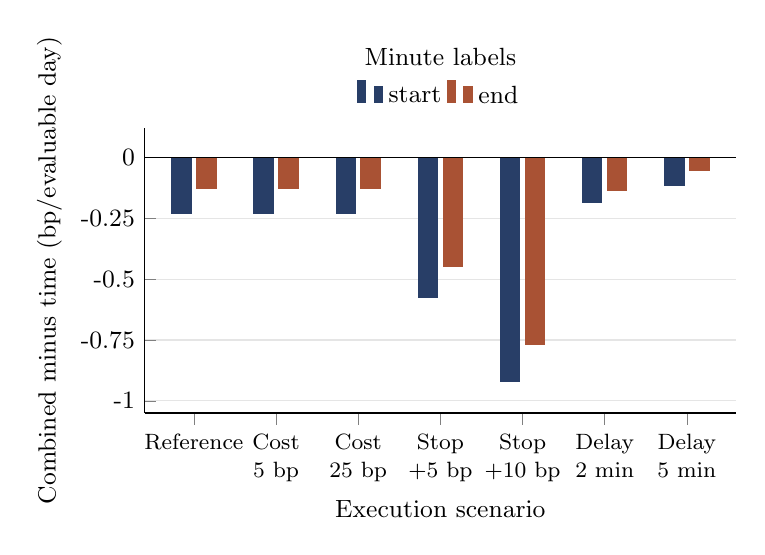
\begin{tikzpicture}
\begin{axis}[
width=0.75\linewidth,height=5.2cm,
ybar,bar width=7pt,
xmin=-0.6,xmax=6.6,ymin=-1.05,ymax=0.12,
xtick={0,1,2,3,4,5,6},
xticklabels={{Reference},{Cost\\5 bp},{Cost\\25 bp},{Stop\\+5 bp},{Stop\\+10 bp},{Delay\\2 min},{Delay\\5 min}},
x tick label style={font=\fontsize{8.5}{10}\selectfont,align=center},
y tick label style={font=\small},
ytick={-1,-0.75,-0.5,-0.25,0},
yticklabels={{\char45{}\allowbreak{}1},{\char45{}\allowbreak{}0.75},{\char45{}\allowbreak{}0.5},{\char45{}\allowbreak{}0.25},{0}},
scaled y ticks=false,
ylabel={Combined minus time (bp/evaluable day)},
ylabel style={align=center,font=\small},
xlabel={Execution scenario},xlabel style={font=\small},
ymajorgrids=true,grid style={gray!20},
axis x line*=bottom,axis y line*=left,
legend style={at={(0.5,1.03)},anchor=south,draw=none,font=\small},
legend columns=2,legend entries={{start},{end}},
title={Minute labels},title style={font=\small,yshift=13pt},
]
\addplot[fill=StartColour,draw=StartColour] coordinates {(0,-0.23247870094142048) (1,-0.23247870094142042) (2,-0.2324787009414204) (3,-0.5769231453858609) (4,-0.9213675898303175) (5,-0.18401247913573263) (6,-0.11507160284811925)};
\addplot[fill=EndColour,draw=EndColour] coordinates {(0,-0.12732863740261363) (1,-0.12732863740261363) (2,-0.12732863740261363) (3,-0.44885094711391504) (4,-0.7703732568251972) (5,-0.13599521891106853) (6,-0.05515904296995816)};
\draw[black,thin] (axis cs:-0.6,0)--(axis cs:6.6,0);
\end{axis}
\end{tikzpicture}
\par\smallskip{\small\RaggedRight Figure 3. Combined minus time mean effects for the declared execution scenarios. The following comparisons are aligned on reference and stressed dates within each interpretation of the timestamps. The Y axis is basis points (bps) of reference capital per evaluable day. The figures plotted are point estimates, not confidence intervals, and these are development comparisons.\par}
\end{minipage}\par\addvspace{8pt}

\par\addvspace{8pt}\noindent\begin{minipage}{\linewidth}
\textbf{Table 14. Funded drawdown for development on reference execution}\par\vspace{5pt}
\begingroup\fontsize{9.5}{11.7}\selectfont
\renewcommand{\arraystretch}{1.12}
\setlength{\tablecontentwidth}{\dimexpr\linewidth-8\tabcolsep\relax}
\noindent\begin{tabular}{@{}>{\RaggedRight\arraybackslash}p{0.23\tablecontentwidth}>{\RaggedRight\arraybackslash}p{0.22\tablecontentwidth}>{\RaggedRight\arraybackslash}p{0.21\tablecontentwidth}>{\RaggedRight\arraybackslash}p{0.14\tablecontentwidth}>{\RaggedRight\arraybackslash}p{0.2\tablecontentwidth}@{}}
\toprule
\textbf{Minute labels / policy} & \textbf{Maximum drawdown (\%) at minute and boundary marks} & \textbf{Daily\char45{}\allowbreak{}close maximum drawdown (\%)} & \textbf{Identified daily closes} & \textbf{The most recent date with an identified daily close.} \\[3pt]
\midrule
Start: Time\char45{}\allowbreak{}only & 9.4282 & 9.3359 & 443 & 2022\char45{}\allowbreak{}10\char45{}\allowbreak{}17 \\[3pt]
Start: Stop\char45{}\allowbreak{}only & 10.4371 & 10.3714 & 443 & 2022\char45{}\allowbreak{}10\char45{}\allowbreak{}17 \\[3pt]
Start: Combined & 10.1413 & 10.1191 & 443 & 2022\char45{}\allowbreak{}10\char45{}\allowbreak{}17 \\[3pt]
End: Time\char45{}\allowbreak{}only & 9.9072 & 9.8252 & 443 & 2022\char45{}\allowbreak{}10\char45{}\allowbreak{}17 \\[3pt]
End: Stop\char45{}\allowbreak{}only & 10.1650 & 10.0845 & 443 & 2022\char45{}\allowbreak{}10\char45{}\allowbreak{}17 \\[3pt]
End: Combined & 10.0296 & 10.0116 & 443 & 2022\char45{}\allowbreak{}10\char45{}\allowbreak{}17 \\[3pt]
\bottomrule\end{tabular}
\endgroup
\par\smallskip{\small\noindent Source: funded\_drawdown.csv, O-L-H-C reference accounts, 1 January 2021 to 17 October 2022. Each account is one segment starting at C0, with 443 identified daily closes and no early ending.\par}
\end{minipage}\par\addvspace{8pt}

{\small\noindent The synthetic coverage check in Table 8 (Appendix B) gives 78.5 to 94.5\% coverage for nominal 95\% intervals, which is why all intervals in this report are treated as exploratory.\par}

\subsection*{F.2 Validation (18 October 2022 to 25 May 2023, 148 sessions)}

\par\addvspace{8pt}\noindent\begin{minipage}{\linewidth}
\textbf{Table 15. Validation returns and risk at reference execution}\par\vspace{5pt}
\begingroup\fontsize{9.5}{11.7}\selectfont
\renewcommand{\arraystretch}{1.12}
\setlength{\tablecontentwidth}{\dimexpr\linewidth-8\tabcolsep\relax}
\noindent\begin{tabular}{@{}>{\RaggedRight\arraybackslash}p{0.25\tablecontentwidth}>{\RaggedRight\arraybackslash}p{0.16\tablecontentwidth}>{\RaggedRight\arraybackslash}p{0.16\tablecontentwidth}>{\RaggedRight\arraybackslash}p{0.225\tablecontentwidth}>{\RaggedRight\arraybackslash}p{0.205\tablecontentwidth}@{}}
\toprule
\textbf{Labels / exit} & \textbf{Mean (bp/day)} & \textbf{ES97.5 (bp)} & \textbf{Minute / boundary MDD (\%)} & \textbf{Daily-close MDD (\%)} \\[3pt]
\midrule
Start / Time & -2.0100 & 13.3647 & 3.0080 & 2.9851 \\[3pt]
Start / Stop & -2.2864 & 11.6941 & 3.4170 & 3.3891 \\[3pt]
Start / Combined & -2.6985 & 11.8599 & 4.0344 & 4.0140 \\[3pt]
End / Time & -2.0510 & 13.9353 & 3.0476 & 3.0354 \\[3pt]
End / Stop & -2.4511 & 11.8667 & 3.6397 & 3.6276 \\[3pt]
End / Combined. & -2.4365 & 12.0332 & 3.6181 & 3.6060 \\[3pt]
\bottomrule\end{tabular}
\endgroup
\end{minipage}\par\addvspace{8pt}

{\small\noindent Each ES rests on 3.70 days of tail weight. One ambiguous episode (end labels, 1 of 260) turns one stop exit into a target exit and leaves the ranking unchanged.\par}

\par\addvspace{8pt}\noindent\begin{minipage}{\linewidth}\centering
\includegraphics[width=0.78\linewidth]{\figfile{validation_funded_equity.png}}
\par\smallskip{\small\RaggedRight Figure 4. Validation funded equity in INR (top) and drawdown in percent (bottom) for the three exits under start and end labels, reference execution. Source: funded\_drawdown.csv.\par}
\end{minipage}\par\addvspace{8pt}

\par\addvspace{8pt}\noindent\begin{minipage}{\linewidth}
\textbf{Table 16. Validation execution sensitivity}\par\vspace{5pt}
\begingroup\fontsize{9.5}{11.7}\selectfont
\renewcommand{\arraystretch}{1.12}
\setlength{\tablecontentwidth}{\dimexpr\linewidth-4\tabcolsep\relax}
\noindent\begin{tabular}{@{}>{\RaggedRight\arraybackslash}p{0.5\tablecontentwidth}>{\RaggedRight\arraybackslash}p{0.25\tablecontentwidth}>{\RaggedRight\arraybackslash}p{0.25\tablecontentwidth}@{}}
\toprule
\textbf{One changed assumption} & \textbf{Start labels (bp/day)} & \textbf{End labels (bp/day)} \\[3pt]
\midrule
Reference & -0.6885 & -0.3855 \\[3pt]
5 bp round-trip cost & -0.6885 & -0.3855 \\[3pt]
25 bp round-trip cost & -0.6885 & -0.3855 \\[3pt]
Extra slip on stops: 5 bp & -1.0838 & -0.7335 \\[3pt]
Extra stop slippage: 10 bp & -1.4790 & -1.0815 \\[3pt]
Entry delay: 2 minutes & -0.2592 & -0.2919 \\[3pt]
Entry delay: 5 minutes & -0.4418 & -0.1920 \\[3pt]
\bottomrule\end{tabular}
\endgroup
\end{minipage}\par\addvspace{8pt}

\subsection*{F.3 Peer-review diagnostics from stored aggregates}

{\small\noindent Recomputed from the saved development and validation exports; no setting was changed.\par}

\par\addvspace{8pt}\noindent\begin{minipage}{\linewidth}
\textbf{Table 17. Calendar, estimation and funded-account samples}\par\vspace{5pt}
\begingroup\fontsize{9.2}{11.2}\selectfont\renewcommand{\arraystretch}{1.12}
\setlength{\tablecontentwidth}{\dimexpr\linewidth-10\tabcolsep\relax}
\noindent\begin{tabular}{@{}>{\RaggedRight\arraybackslash}p{0.27\tablecontentwidth}>{\RaggedRight\arraybackslash}p{0.12\tablecontentwidth}>{\RaggedRight\arraybackslash}p{0.15\tablecontentwidth}>{\RaggedRight\arraybackslash}p{0.18\tablecontentwidth}>{\RaggedRight\arraybackslash}p{0.13\tablecontentwidth}>{\RaggedRight\arraybackslash}p{0.15\tablecontentwidth}@{}}\toprule
\textbf{Stage / label} & \textbf{Sched.} & \textbf{Complete} & \textbf{Unavailable} & \textbf{Funded} & \textbf{Episodes} \\[3pt]\midrule
Development / start & 443 & 360 & 83 & 443 & 637 \\[3pt]
Development / end & 443 & 381 & 62 & 443 & 662 \\[3pt]
Validation / start & 148 & 148 & 0 & 148 & 266 \\[3pt]
Validation / end & 148 & 148 & 0 & 148 & 260 \\[3pt]
Final / start & 148 & 88 & 60 & 148 & 160 \\[3pt]
Final / end & 148 & 88 & 60 & 148 & 170 \\[3pt]
\bottomrule\end{tabular}\endgroup\end{minipage}\par\addvspace{8pt}
{\small\noindent Scheduled, complete-case and funded dates are different counts. The 83 and 62 unavailable development dates are one explicit exclusion plus 82 and 61 incomplete candidates; a funded account can remain identified on a date with no eligible entry. The 21-date gap between timestamp conventions arises because one missing observation invalidates later twenty-session windows, and a one-minute shift changes which observations fall at window edges; it is not attributable to a single outage and does not occur in validation. In the final test the 60 unavailable dates are the declared gaps of 23 June, 20 July and 22 September 2023 and the twenty sessions after each; the September and October minute gaps fell outside every signal window, so the count matches the higher of the two figures declared before the freeze, under both conventions.\par}

\par\addvspace{8pt}\noindent\begin{minipage}{\linewidth}
\textbf{Table 18. Development combined-minus-time sensitivity}\par\vspace{5pt}
\begingroup\fontsize{9.2}{11.2}\selectfont\renewcommand{\arraystretch}{1.12}
\setlength{\tablecontentwidth}{\dimexpr\linewidth-8\tabcolsep\relax}
\noindent\begin{tabular}{@{}>{\RaggedRight\arraybackslash}p{0.32\tablecontentwidth}>{\RaggedRight\arraybackslash}p{0.2\tablecontentwidth}>{\RaggedRight\arraybackslash}p{0.14\tablecontentwidth}>{\RaggedRight\arraybackslash}p{0.2\tablecontentwidth}>{\RaggedRight\arraybackslash}p{0.14\tablecontentwidth}@{}}\toprule
\textbf{Setting} & \textbf{Start bp/day} & \textbf{Start days} & \textbf{End bp/day} & \textbf{End days} \\[3pt]\midrule
Reference & -0.2325 & 360 & -0.1273 & 381 \\[3pt]
Cost: 5 bp & -0.2325 & 360 & -0.1273 & 381 \\[3pt]
Cost: 25 bp & -0.2325 & 360 & -0.1273 & 381 \\[3pt]
Stop slippage: 5 bp & -0.5769 & 360 & -0.4489 & 381 \\[3pt]
Stop slippage: 10 bp & -0.9214 & 360 & -0.7704 & 381 \\[3pt]
Entry delay: 2 min & -0.1840 & 360 & -0.1360 & 381 \\[3pt]
Entry delay: 5 min & -0.1151 & 360 & -0.0552 & 381 \\[3pt]
\bottomrule\end{tabular}\endgroup\end{minipage}\par\addvspace{8pt}
{\small\noindent Each comparison uses the dates common to the scenario and reference execution (360 and 381 in development, 148 in validation), and the combined-minus-time contrast is negative in every setting.\par}

\par\addvspace{8pt}\noindent\begin{minipage}{\linewidth}
\textbf{Table 19. Expected-shortfall sensitivity to removing one day}\par\vspace{5pt}
\begingroup\fontsize{9.2}{11.2}\selectfont\renewcommand{\arraystretch}{1.12}
\setlength{\tablecontentwidth}{\dimexpr\linewidth-8\tabcolsep\relax}
\noindent\begin{tabular}{@{}>{\RaggedRight\arraybackslash}p{0.24\tablecontentwidth}>{\RaggedRight\arraybackslash}p{0.16\tablecontentwidth}>{\RaggedRight\arraybackslash}p{0.15\tablecontentwidth}>{\RaggedRight\arraybackslash}p{0.16\tablecontentwidth}>{\RaggedRight\arraybackslash}p{0.29\tablecontentwidth}@{}}\toprule
\textbf{Stage / label} & \textbf{Policy} & \textbf{Tail days} & \textbf{ES97.5 bp} & \textbf{Leave-one-day-out bp} \\[3pt]\midrule
Dev. / start & Time & 9.0000 & 17.4085 & 14.9946--17.4221 \\[3pt]
Dev. / start & Stop & 9.0000 & 14.8495 & 14.3377--14.8540 \\[3pt]
Dev. / start & Combined & 9.0000 & 14.4075 & 13.7943--14.4125 \\[3pt]
Dev. / end & Time & 9.5250 & 15.3083 & 14.1607--15.3189 \\[3pt]
Dev. / end & Stop & 9.5250 & 14.2981 & 13.2745--14.3044 \\[3pt]
Dev. / end & Combined & 9.5250 & 13.2774 & 12.1298--13.2850 \\[3pt]
Val. / start & Time & 3.7000 & 13.3647 & 11.8750--13.3811 \\[3pt]
Val. / start & Stop & 3.7000 & 11.6941 & 11.1532--11.6987 \\[3pt]
Val. / start & Combined & 3.7000 & 11.8599 & 11.2186--11.8669 \\[3pt]
Val. / end & Time & 3.7000 & 13.9353 & 12.0263--13.9584 \\[3pt]
Val. / end & Stop & 3.7000 & 11.8667 & 11.4177--11.8717 \\[3pt]
Val. / end & Combined & 3.7000 & 12.0332 & 11.4182--12.0384 \\[3pt]
Final / start & Time & 2.2000 & 16.2041 & 13.1231--16.2502 \\[3pt]
Final / start & Stop & 2.2000 & 15.8260 & 14.7903--15.8374 \\[3pt]
Final / start & Combined & 2.2000 & 16.0851 & 15.5336--16.0909 \\[3pt]
Final / end & Time & 2.2000 & 13.6629 & 13.2718--13.6651 \\[3pt]
Final / end & Stop & 2.2000 & 13.4155 & 12.3667--13.4319 \\[3pt]
Final / end & Combined & 2.2000 & 13.3516 & 11.9713--13.3753 \\[3pt]
\bottomrule\end{tabular}\endgroup\end{minipage}\par\addvspace{8pt}
{\small\noindent The last column gives the minimum and maximum ES97.5 when each day is deleted in turn and the tail mass recomputed; it is a sensitivity range, not a confidence interval. The 3.7-day tail in validation and the 2.2-day tail in the final test call for particular caution.\par}

{\small\noindent Table 20 removes, for each stage and label, the date with the largest combined loss across the three exits and recomputes the contrast and ES. Where that date's neighbours are not in the saved tail records, ES is shown as a range.\par}

\par\addvspace{8pt}\noindent\begin{minipage}{\linewidth}
\textbf{Table 20. Rankings after removing the worst shared date}\par\vspace{5pt}
\begingroup\fontsize{9.2}{11.2}\selectfont\renewcommand{\arraystretch}{1.12}
\noindent\begin{tabular}{@{}>{\RaggedRight\arraybackslash}p{2.3cm}>{\RaggedRight\arraybackslash}p{1.8cm}rrrr@{}}\toprule
\textbf{Stage / label} & \textbf{Date removed} & \textbf{\makecell{Combined$-$time\\before}} & \textbf{\makecell{Combined$-$time\\after}} & \textbf{\makecell{Time-only ES\\after}} & \textbf{\makecell{Combined ES\\after}} \\[3pt]\midrule
Dev. / start & 2022-04-19 & $-0.2325$ & $-0.2894$ & 14.995 & 14.189 \\[3pt]
Dev. / end & 2021-07-07 & $-0.1273$ & $-0.1529$ & 13.57--14.16 & 12.49--13.04 \\[3pt]
Val. / start & 2022-12-09 & $-0.6885$ & $-0.7250$ & 10.13--12.14 & 9.88--11.92 \\[3pt]
Val. / end & 2022-12-09 & $-0.3855$ & $-0.4113$ & 10.75--12.69 & 9.83--11.90 \\[3pt]
Final / start & 2023-12-08 & $-0.0850$ & $-0.1138$ & 12.14--13.12 & 14.38--15.63 \\[3pt]
Final / end & 2023-09-13 & $-0.0478$ & $-0.0439$ & 12.40--13.49 & 11.10--12.01 \\[3pt]
\bottomrule\end{tabular}\endgroup\end{minipage}\par\addvspace{8pt}
{\small\noindent Time-only stays ahead on the mean in all six cases. Under final start labels the combined exit's ES advantage reverses once 8 December 2023 is removed.\par}

\end{document}
